%%% Template for class notes
%%% Created by Daniel Campos based on the template by Willian Chamma,
%%% which was based on the template by Mikhail Klassen

\documentclass[12pt,a4paper, brazil]{article}

%%%%%%% HEADER INFORMATION
\newcommand{\workingDate}{\textsc{\selectlanguage{english}\today}}
\newcommand{\userName}{Course 25/26}
\newcommand{\institution}{UAL}
\usepackage{researchdiary_png}
\usepackage{tcolorbox}

\begin{document}

\begin{center}
{\textbf {\Large Lab 3: Router Firmware Analysis}}\\[5mm]
{\large } \\[5mm]
\today\\[5mm] %% optional date
\end{center}

\section{Hardware Security Analysis}

Our daily environment is full of digital devices, and therefore they are susceptible to attacks. How can we prevent any of the devices that surround us in our daily lives—at home, work, university, on the bus, in the car, etc.—from becoming a threat to our integrity, security, and privacy? The answer is to reach the vulnerability before someone else does to exploit it for their own benefit. One example of the most vulnerable devices, which rarely undergo security audits (from a firmware perspective), are routers. Figure~\ref{fig:router} shows a TP-LINK router like those commonly found in SMEs, homes, etc. This document aims to show how to extract and analyze the firmware of an embedded system.

\begin{figure}[htpb]
    \centering
    \caption{TP-LINK Router.}
    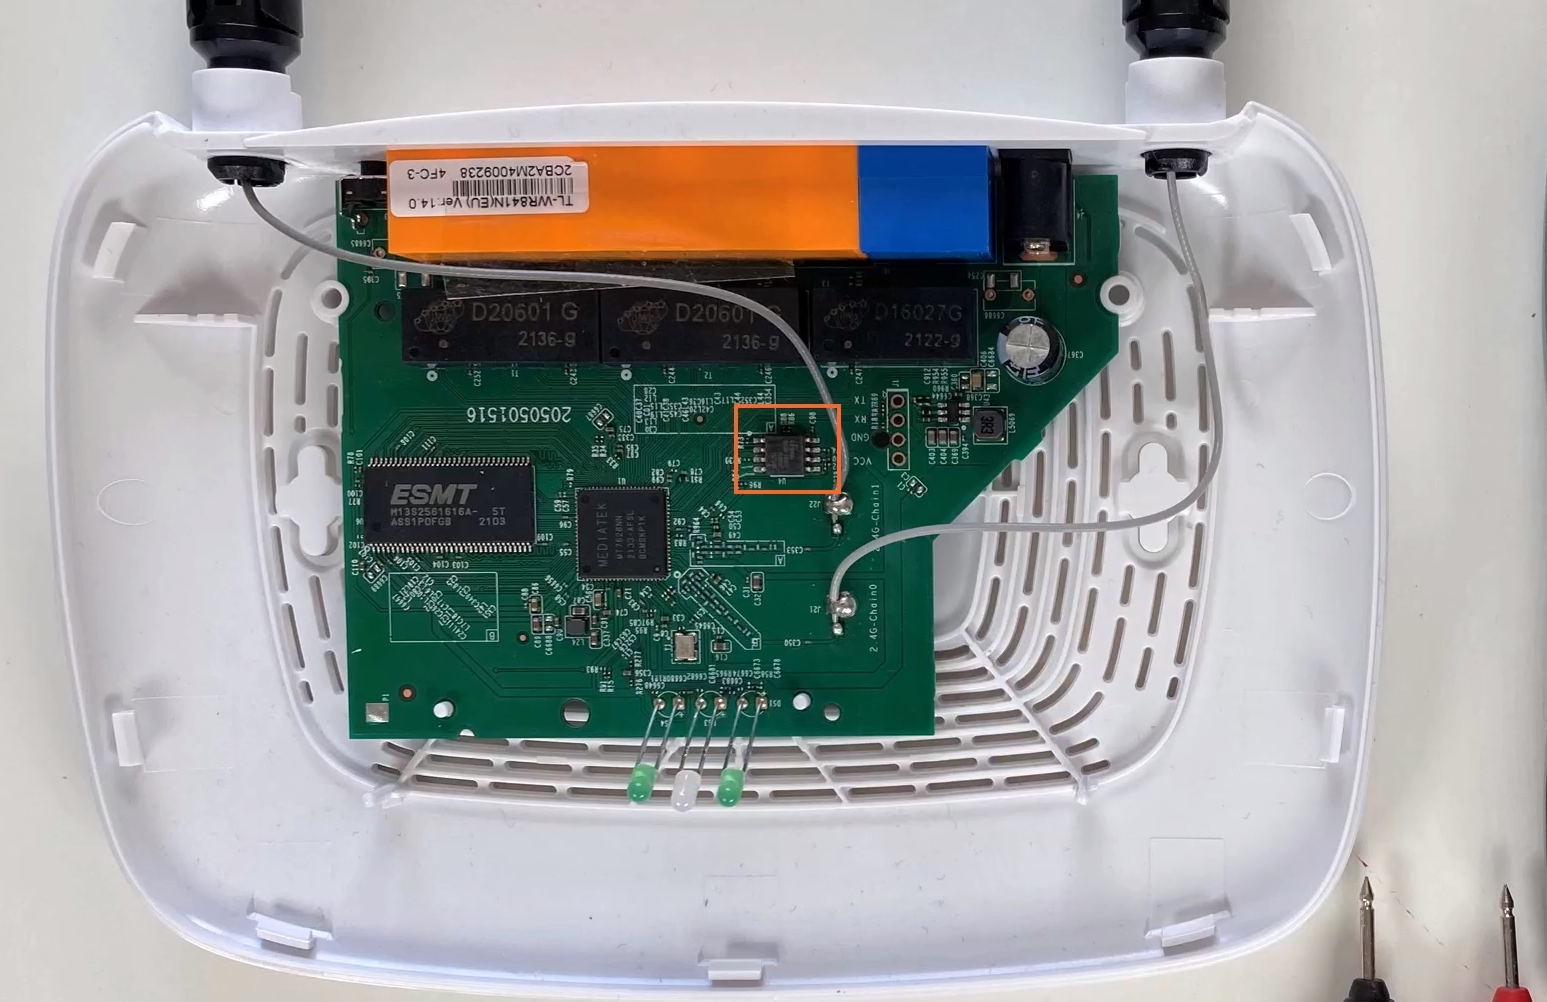
\includegraphics[scale=.2]{imagenes/1_router.png}
    \label{fig:router}
\end{figure}

The goal is to study whether there are opportunities for data exfiltration or threats while using the device. The basic components we will work with are shown in Figure~\ref{fig:accesorouter}, where you can see the elements used to extract the firmware.

\begin{figure}[htpb]
    \centering
    \caption{Access to the router.}
    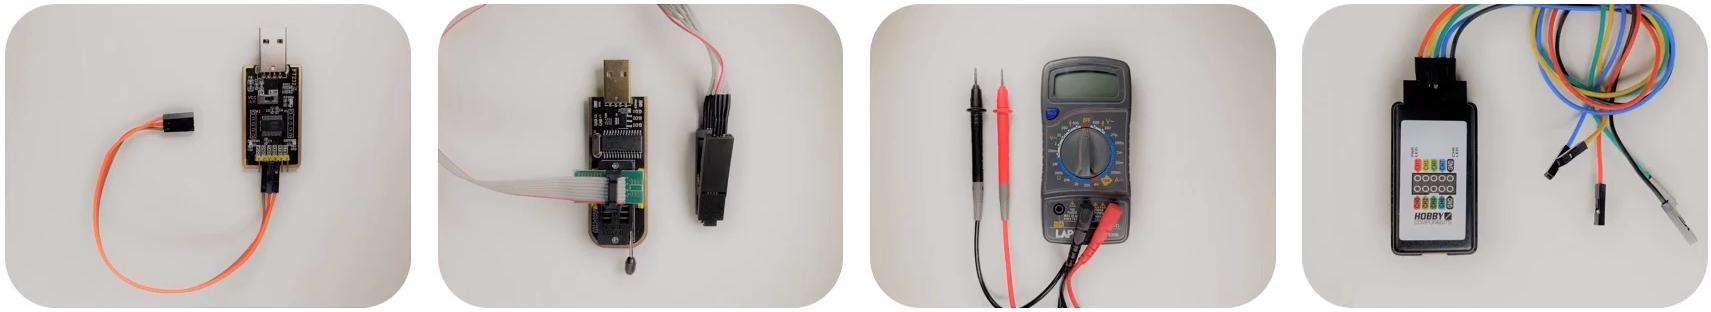
\includegraphics[scale=.25]{imagenes/1_accesorouter.png}
    \label{fig:accesorouter}
\end{figure}

In Figure~\ref{fig:router}, we have intentionally marked one of the three chips present in this device. Later, we will discuss the problems we encountered and the tools we discarded or successfully used. When facing a device like this, the first step is to identify the components and the communication interfaces they use. For this, documentation is necessary. So, depending on the communication interfaces the device offers, we will use some techniques (slower ones, such as UART access or debugging ports) or faster ones to try to access what we are interested in: \emph{\textcolor{red}{firmware}}.

Once we have extracted the data from the device, the next step is to understand the format of the binary information obtained. That is: is it encrypted? What structure does it follow? How can we open the binary package we just—hopefully—extracted from the router? For this, we will use a set of tools (file carving, etc.) to try to understand what kind of data we are dealing with and extract useful information such as the kernel and the root file system (rootfs).

The final stage of this lab involves using reverse engineering (explained in the chapter titled \emph{\textcolor{red}{reversing}}; in this case we chose \emph{\textcolor{red}{Ghidra}} over IDA) to extract useful information such as \emph{usernames, passwords or password hashes, encryption keys, etc.} in order to identify vulnerabilities we might exploit. It is important to note that all these devices have internal servers that allow users to configure them, and such software is likely to contain flaws.

\subsection{Hardware-Based Attacks}

We are all aware that application development can involve programming errors (from the perspective of \emph{\textcolor{red}{secure coding}}), which may lead to unauthorized access. We have studied this in subjects such as \emph{Programming and Software Engineering}. However, hardware is also a key component. As we learned in \emph{Peripherals and Interfaces}, a cryptosystem may be theoretically unbreakable, but its careless implementation in a SoC\footnote{System on Chip: a device that includes processing cores, memory (SRAM, DRAM, flash), and microcontrollers, all in the same package.} may expose it and make it vulnerable.

Penetration testing or \emph{pentesting} is well known in the security community and is typically focused on networks and servers. But hardware devices are also part of the chain that should undergo pentesting. In this case, the aim is to analyze or locate vulnerabilities and assess the hardware’s capacity to prevent unauthorized access through physical interactions with the device. The procedure always suggests that the device be \textbf{disassembled} (which may void the warranty) and that we identify where the debugging and/or communication interfaces are located, so we can interact with them at a low level. What is the purpose of this?

\begin{itemize}
    \item Analyze whether the device might reveal sensitive information: passwords, encryption keys, hashes stored in the \emph{flash} memory. Or whether we are able to capture this information while it is being transmitted internally across the system buses.
    \item Analyze whether the device allows privilege escalation: this involves analyzing the software running on the device and seeing if we can exploit moments when the software needs privileged access.
    \item Analyze whether, after gaining access to this device, we can compromise others that depend on it. This is known as \emph{pivoting and lateral movement}.
\end{itemize}

The plethora of devices around us is immense and constantly growing (as shown in Figure~\ref{fig:iot}). Manufacturers, pressured by TTM (Time To Market), rarely harden the firmware of their devices, making both them and the ecosystem they connect to extremely vulnerable.

\begin{figure}[htpb]
    \centering
    \caption{Growing ecosystem of devices.}
    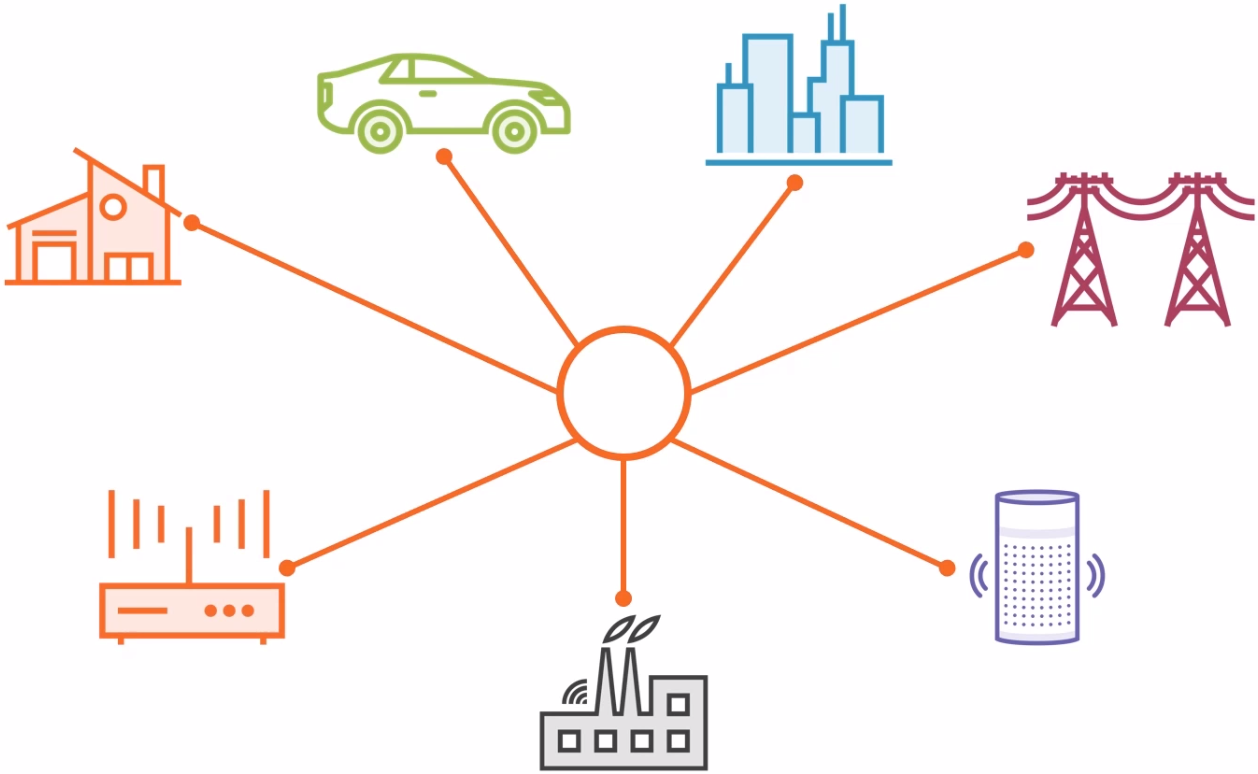
\includegraphics[scale=.25]{imagenes/1_ioT.png}
    \label{fig:iot}
\end{figure}

All these devices are (and we can assume will continue to be) susceptible to attacks. Therefore, having techniques to analyze them and verify their protection capacity is fundamental. Many of these devices use software that requires internet connectivity (and corporate cloud connections) so that the user—whether an end-user or a company technician—can manage the device using web interfaces. This further increases the exposure and attack surface.

Additionally, these devices may communicate through a wide variety of channels (Wi-Fi, Bluetooth, NFC, GSM, SMS, etc.), each with known weaknesses and vulnerabilities, which will surely be used against the integrity of our device and the data it protects. In this project, we will conduct our analysis from the physical layer, not from applications and network protocols, which are the usual domain of \emph{penetration tests}. Through the hardware layer, we will attempt to extract sensitive information from the device's configuration itself (see Figure~\ref{fig:ini}).

\begin{figure}[htpb]
    \centering
    \caption{Access through the hardware layer.}
    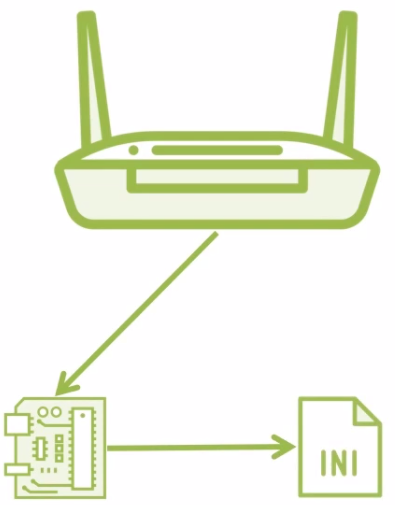
\includegraphics[scale=.3]{imagenes/1_ini.png}
    \label{fig:ini}
\end{figure}

\subsection{Component Identification}

As we noted in the previous section, this type of study requires disassembling the device. But how do we know what's connected inside? What are those chips?

To carry out this task, we will use a modern router, purchased via \emph{Amazon}, commonly found in homes and small shops. The router we will work with is the \textbf{TL-WR841N}, as shown in Figure~\ref{fig:router} and as it comes (without disassembly) in Figure~\ref{fig:routerTapa}:

\begin{figure}[htpb]
    \centering
    \caption{TL-WR841N}
    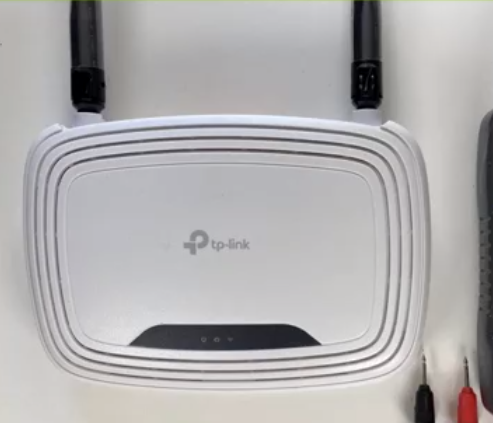
\includegraphics[scale=.4]{imagenes/1_routerTapa}
    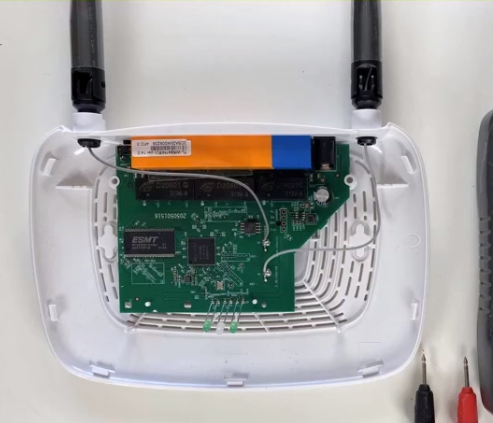
\includegraphics[scale=.4]{imagenes/1_routerTapa2}
    \label{fig:routerTapa}
\end{figure}

It is a 300Mbps router with wired (Ethernet) and wireless (Wi-Fi) interfaces. We chose this device for several reasons: first, because of the \textbf{SoC} it includes (discussed later in the components section); second, due to its technical capabilities, it is used in many environments (especially small businesses); and lastly, because of its price—if the analysis disables the device, the loss is not significant.

To access the board, we need to remove two screws on the bottom of the device. Then, we must carefully remove the cover, which is held by plastic tabs. \textbf{\textcolor{red}{In most cases, analyzing a device as we intend to do will void the warranty, and this should be documented if the analysis is to be performed for third parties.}} Furthermore, interacting with the circuitry of a device can damage it due to electrostatic discharge, accidental short circuits, applying more voltage than it supports, etc. That’s why it's helpful to have a multimeter and the device's datasheet on hand.

Upon lifting the cover, several components are visible:

\begin{itemize}
    \item \textbf{Ethernet (orange) and WAN (blue) port bank}. These provide the device's wired connectivity. See Figure~\ref{fig:ethernet}.
    \item \textbf{Power supply of the device}, which in this case is a 9V DC input. See Figure~\ref{fig:vcc}.
    \item \textbf{Serial interface}, used for device debugging. It consists of four pins (\emph{transmit (TX)}, \emph{receive (RX)}, \emph{ground (GND)}, and \emph{power (Vcc)}). It's uncommon for debugging interfaces to be labeled. In this case, they are, which helps us—but we will analyze them as if they were not labeled to understand how to identify each pin. See Figure~\ref{fig:depuracion}.
    \item In Figure~\ref{fig:8bflash}, we can see a marked 8-pin serial flash memory chip with a capacity of 32 Mb. It features a serial interface for communication. \textbf{\textcolor{red}{This chip is where we will find the system firmware stored}}. In a simple device like our router, the \textbf{firmware} (\textbf{\textcolor{blue}{its role and importance have been explained in previous sections}}) provides the operating system for the device. In more complex systems like PCs or laptops, firmware only handles boot and system loading phases, offering an abstraction layer.
    \item \textbf{MediaTek MT7628 System On Chip (SoC)}. \textbf{\textcolor{red}{This SoC was one of the first specifically designed and developed for home routers and IoT gateways\footnote{This is especially relevant.}}} It essentially combines an 802.11 Wi-Fi radio with a MIPS processor running at 580 MHz.
    \item Figure~\ref{fig:memoria} shows the last relevant component: a 4MB DDR SD-RAM chip. When the device boots, the firmware loads the operating system from flash memory into RAM (as explained in the firmware section). This process is known as \emph{shadowing}. The OS remains in RAM until the system is powered off.
\end{itemize}

\begin{figure}[htpb]
    \centering
    \caption{Ethernet port bank}
    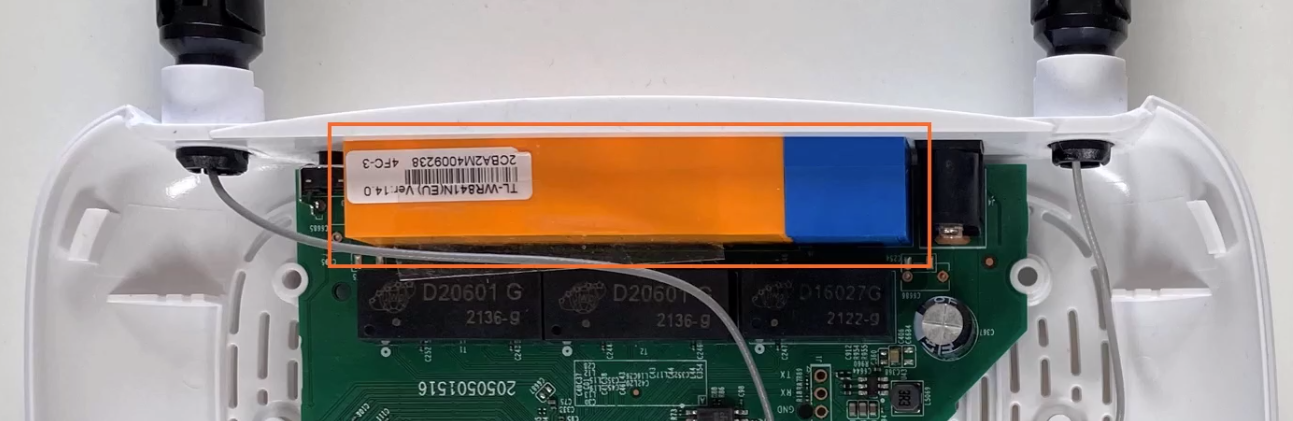
\includegraphics[scale=.4]{imagenes/1_ethernet.png}
    \label{fig:ethernet}
\end{figure}

\begin{figure}[htpb]
    \centering
    \caption{Power supply: 9 volts}
    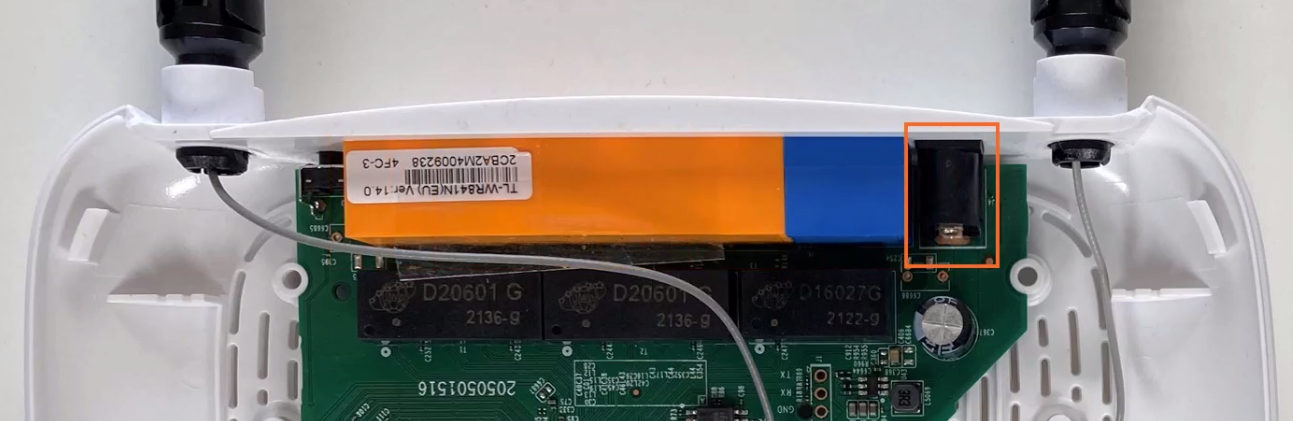
\includegraphics[scale=.4]{imagenes/1_vcc.png}
    \label{fig:vcc}
\end{figure}

\begin{figure}[htpb]
    \centering
    \caption{Serial debug interface}
    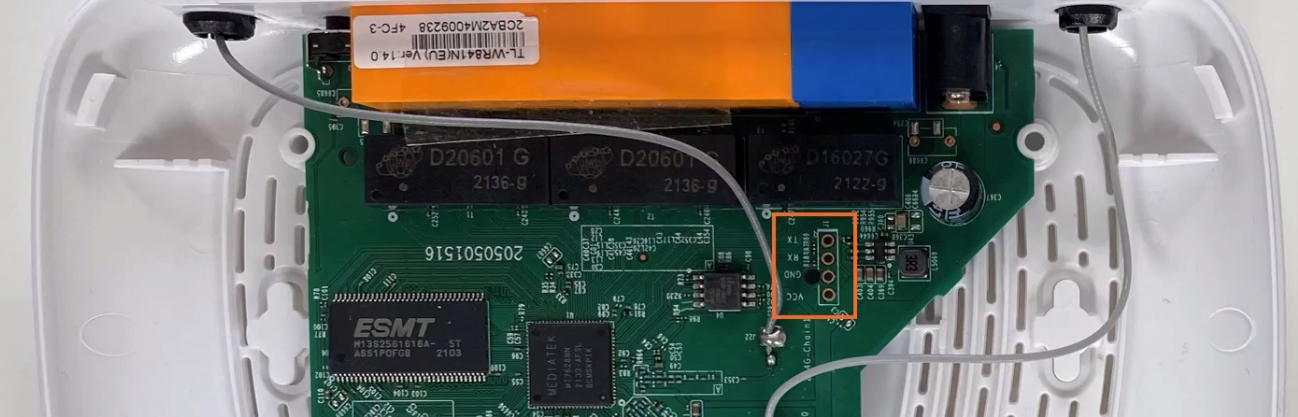
\includegraphics[scale=.4]{imagenes/1_depuracion.png}
    \label{fig:depuracion}
\end{figure}

\begin{figure}[htpb]
    \centering
    \caption{Serial flash memory, 8-bit. Firmware location.}
    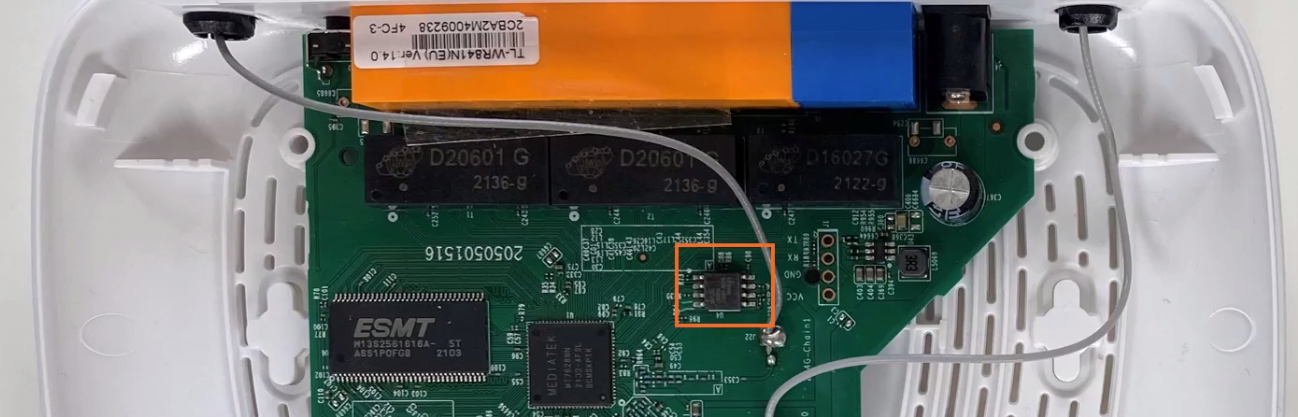
\includegraphics[scale=.4]{imagenes/1_8bflash.png}
    \label{fig:8bflash}
\end{figure}

\begin{figure}[htpb]
    \centering
    \caption{MediaTek MT7628 System On Chip (SoC).}
    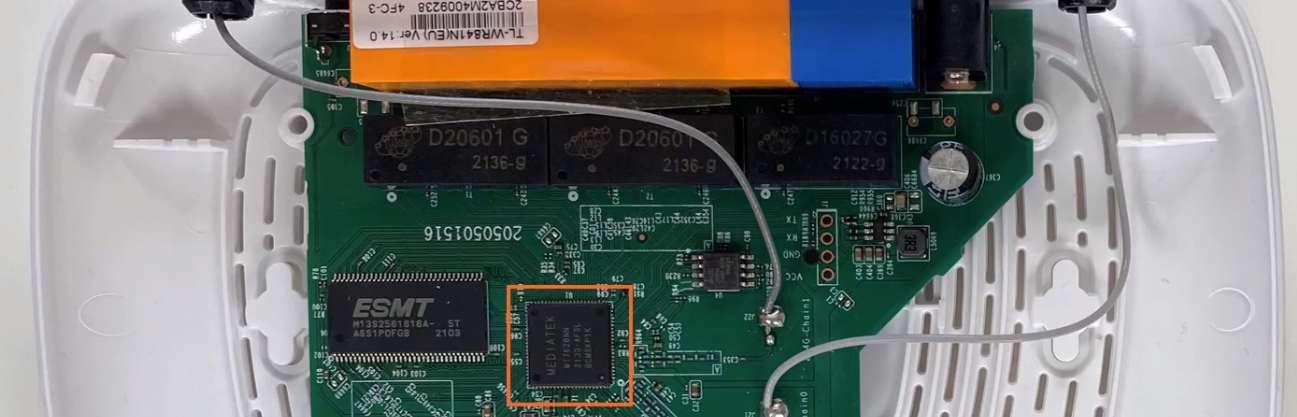
\includegraphics[scale=.4]{imagenes/1_soc.png}
    \label{fig:soc}
\end{figure}

\begin{figure}[htpb]
    \centering
    \caption{System memory. 4MB DDR Elite SD-RAM}
    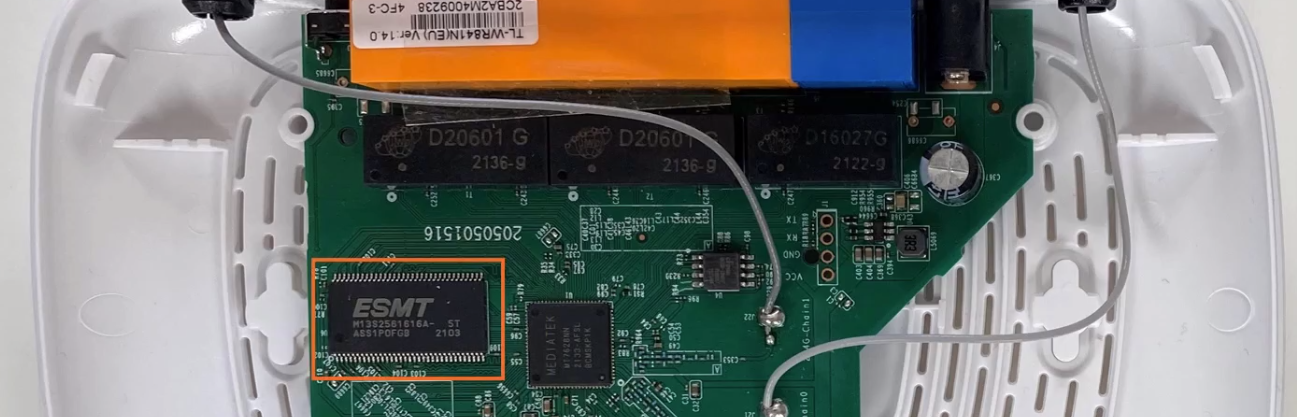
\includegraphics[scale=.4]{imagenes/1_memoria.png}
    \label{fig:memoria}
\end{figure}

Obviously, just by looking at the chips after removing the cover, it’s impossible to know their brand, model, function, etc. But with magnifiers or magnification, we can extract chip details (Figure~\ref{fig:zoom}), which will allow us to locate their datasheets.

\begin{figure}[htpb]
    \centering
    \caption{Components}
    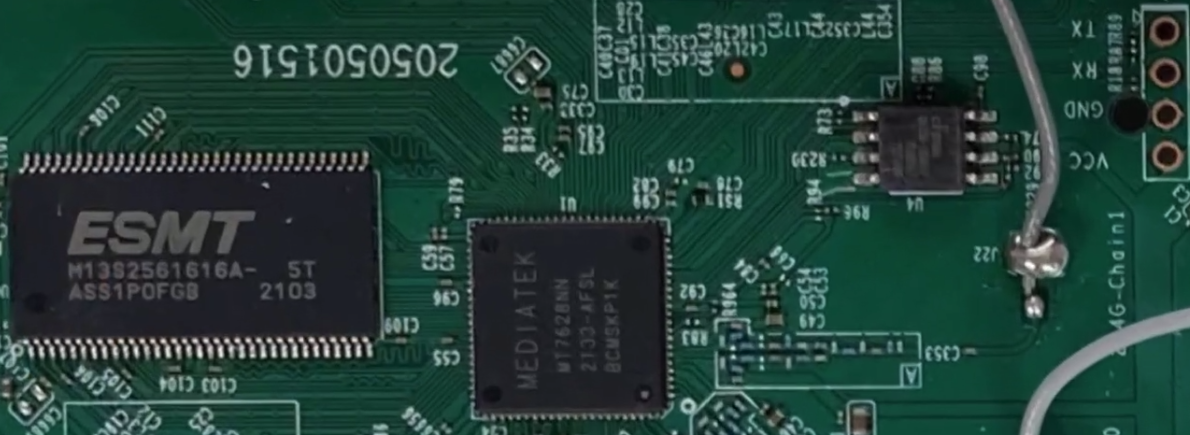
\includegraphics[scale=.4]{imagenes/1_zoom.png}
    \label{fig:zoom}
\end{figure}

\subsubsection{Interfaces}

Once we have identified our core components, the question is: what interfaces do we have to communicate with them? In this router, the debug interface uses the \textbf{UART interface} (Universal Asynchronous Receiver Transmitter). It is a very slow interface. It provides asynchronous serial communication (no clock signal). Therefore, a configuration phase is required to establish speed and data frame format. If we use these pins, we must configure these parameters.

Transmission is carried out through two separate lines (pins): transmit and receive. So we know that the debug interface uses UART. On the other hand, since we have a NOR flash memory, the commonly used interface is SPI, which we confirmed when analyzing the chip type.

\textbf{SPI Interface}: Unlike UART (a circuit within the chip), SPI is a communication protocol following a client-server model. SPI requires four communication lines: one for the client to communicate with the server (MISO), one for the server to communicate with the client (MOSI), one for the clock signal (SCLK), and one to select the server (chip) we want to communicate with (CS).

\textbf{I2C (Inter-Integrated Circuit):} combines the best features of UART and SPI. We can connect several servers to a single client like with SPI, and have several clients controlling one or more servers. Like UART, I2C uses two communication lines (SDA and SCL). SDA (Serial Data line) allows both client and server to send or receive data (half-duplex), while SCL (Serial Clock) carries the synchronization.

\subsection{Tools}

In this section, we will describe the tools we will (or initially thought we would) find useful to communicate with, interrogate, and analyze each hardware component. Considering we have a \textbf{UART interface}, the simplest way to communicate through it is with a USB to TTL cable (Figure~\ref{fig:usbttl}).

\begin{figure}[htpb]
    \centering
    \caption{Tools: USB to TTL (FT232)}
    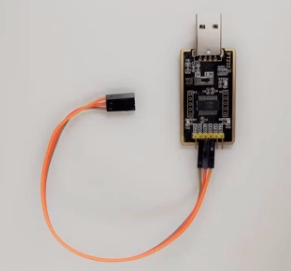
\includegraphics[scale=.6]{imagenes/1_usbttl.png}
    \label{fig:usbttl}
\end{figure}

As seen in Figure~\ref{fig:usbttl}, the cable contains four wires to connect Vcc, GND, TX, and RX. The other end has a USB connector to connect it to a computer.

Another useful tool is the \textbf{flash memory programmer} (Figure~\ref{fig:flash}). This tool allows us to read and/or write to flash memories. In this case, we used a CH341A programmer.

\begin{figure}[htpb]
    \centering
    \caption{Tools: Flash programmer (CH341A).}
    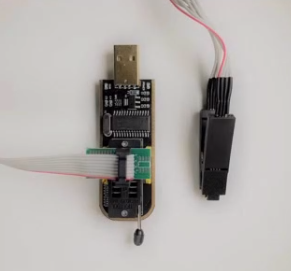
\includegraphics[scale=.6]{imagenes/1_flash.png}
    \label{fig:flash}
\end{figure}

This tool includes a clip to connect to the chip in question. The programmer can write to blank flash memory and even if the chip is removed from the board, it can be read directly by connecting it to the programmer. In this case, we have a small ribbon cable connecting the programmer to an 8-pin circuit (SOIC clip). This clip connects directly to the memory chip, aligning each memory pin with the corresponding pin on the clip.

\textbf{Multimeter}: In Figure~\ref{fig:accesorouter}, all the tools we used are shown, including the multimeter, which everyone is familiar with. In this case, we use the multimeter (specifically that one) to determine which pins to use for receiving and transmitting.

\textbf{Logic Analyzer}: Although we have one, we ultimately didn’t need to use it. It is used for analyzing protocols. Figure~\ref{fig:analizador} shows the analyzer (a very inexpensive one) we have. A logic analyzer is used to analyze signals in a digital system or circuit.

\begin{figure}[htpb]
    \centering
    \caption{Tools: Logic analyzer.}
    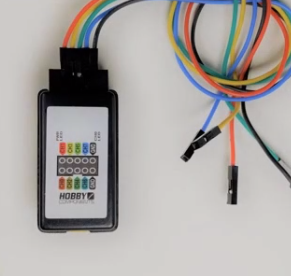
\includegraphics[scale=.6]{imagenes/1_analizador.png}
    \label{fig:analizador}
\end{figure}

The total budget for acquiring these tools did not exceed forty euros. Of course, hardware analysis requires professional tools with much higher costs than the ones we used.

\subsubsection{Software}

Now that we know our device’s architecture, the interfaces we can use to communicate with it, and have a basic toolset, we need to consider what software we can use with each tool to physically connect with our device. There is no one-size-fits-all solution, but this toolkit reflects the feasible options with the tools we have:

\begin{itemize}
    \item \textbf{PuTTY}  
    Open-source terminal emulator. Originally designed for SSH, Telnet, and similar remote administration services, it also supports serial communication. To connect to a device, we must know the transmission speed (baud rate) configured for serial connections. Once we set the correct speed, we can use the emulator to send commands to the device and read responses.
    \begin{figure}[htpb]
    \centering 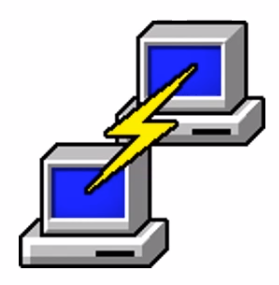
\includegraphics[scale=.15]{imagenes/1_putty.png}
    \end{figure}
    \vspace{-3 mm}

    \item \textbf{Flash ROM}  
    A tool to identify the type of flash, read, write, verify, and even erase flash memory chips. It is especially designed to work with flash memories storing BIOS, EFI, firmware, and other binary images in programmable devices. It can be used with the CH341A programmer to dump firmware from a device’s flash memory.
    \begin{figure}[htpb]
    \centering 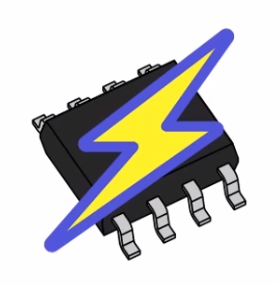
\includegraphics[scale=.15]{imagenes/1_flashrom.png}
    \end{figure}
    \vspace{-3 mm}

    \item \textbf{Binwalk}  
    Once we have the firmware, we must be able to examine the binary (image) we downloaded to start understanding it. Binwalk is a tool for searching embedded files, executables, etc., in a firmware image. It is specifically designed to identify files and embedded code in firmware images. It includes a signature file of common items found in firmware, such as compressed files, firmware headers, Linux kernels, bootloaders, filesystems, etc.
    \begin{figure}[htpb]
    \centering 
\includegraphics[scale=.15]{imagenes/1_binwalk.png}
    \end{figure}
    \vspace{-3 mm}

    \item \textbf{Ghidra}  
    A framework with tools for reverse engineering. It includes a suite of utilities to analyze compiled code through disassembling, assembling, decompilation, scripting, etc. Ghidra supports a wide variety of instruction sets and executable formats and can be used interactively or in headless (automated) mode.
    \begin{figure}[htpb]
    \centering 
\includegraphics[scale=.15]{imagenes/1_ghidra.png}
    \end{figure}
\end{itemize}

\newpage
\subsection{How to Identify the Pins in UART}

This time we were lucky (we didn’t expect the pins to be labeled), but we will still explain the method used to identify which pins are used for TX, RX, GND, and VCC using voltage and resistance measurements with the multimeter. That way, if we encounter a system with a UART interface that is not labeled (see Figure~\ref{fig:interfazUART}), our first option would be to consult the datasheet of the board to see whether it identifies the UART interface and specifies the pins. If that is not available, we will need to take measurements and deduce the function of each pin based on them.

\begin{figure}[htpb]
     \caption{UART Interface: what they look like.}
     \centering
     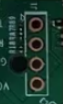
\includegraphics[scale=1]{imagenes/1_UART.png}
     \label{fig:interfazUART}
\end{figure}

In this basic measurement scheme, we have three types of measurements for each pin. The first will be resistance between each pin and ground (GND). This will help us identify the GND pin, which will show zero resistance. The second measurement is the resistance between each pin and VCC, to determine which pin is VCC (the one with zero resistance). The next step is to measure voltage on the pins to try to identify TX and RX.

\begin{table}[htpb]
\centering
\caption{UART Electrical Measurements.}
\label{tab:my-table}
\begin{tabular}{@{}clll@{}}
\toprule
{\color[HTML]{FE0000} \textbf{Pin}} & \multicolumn{1}{c}{{\color[HTML]{FE0000} \textbf{R$_{GND}$}}} & \multicolumn{1}{c}{{\color[HTML]{FE0000} \textbf{R$_{VCC}$}}} & \multicolumn{1}{c}{{\color[HTML]{FE0000} \textbf{V}}} \\ \midrule
\multicolumn{1}{|c|}{\textbf{1}}    &                                                               &                                                               &                                                       \\ \midrule
\multicolumn{1}{|c|}{\textbf{2}}    &                                                               &                                                               &                                                       \\ \midrule
\multicolumn{1}{|c|}{\textbf{3}}    &                                                               &                                                               &                                                       \\ \midrule
\multicolumn{1}{|c|}{\textbf{4}}    &                                                               &                                                               &                                                       \\ \bottomrule
\end{tabular}
\end{table}

For this, we place the black probe on a known ground point (see Figure~\ref{fig:interfazUARTmediciones}, near the reset button—it's a piece of metal used as reference):

\begin{figure}[htpb]
     \caption{UART Interface: GND measurements.}
     \centering
     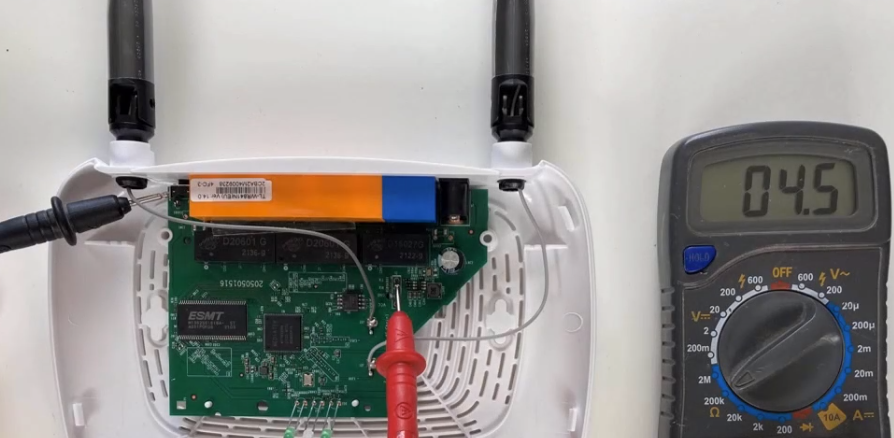
\includegraphics[scale=.4]{imagenes/1_UARTmediciones.png}
     \label{fig:interfazUARTmediciones}
\end{figure}

The red probe is placed on the first UART pin (closest to the Ethernet connector bank). The multimeter is set to measure resistance (200K$\Omega$), and the reading shows \textbf{\textcolor{red}{\emph{0.45k$\Omega$}}}. Repeating the operation with the second pin gives a reading of \textbf{\textcolor{red}{\emph{0.9k$\Omega$}}}. The third pin gives a reading of \textbf{\textcolor{red}{\emph{0.0k$\Omega$}}}, making it the perfect candidate for \textbf{GND}, since there is no resistance between pin 3 and the black probe measurement point (ground). The last pin shows \textbf{\textcolor{red}{\emph{21.6k$\Omega$}}}. The updated measurement table is as follows:

\begin{table}[htpb]
\centering
\caption{UART Electrical Measurements: GND}
\label{tab:gnd}
\begin{tabular}{@{}cccc@{}}
\toprule
{\color[HTML]{FE0000} \textbf{Pin}} & {\color[HTML]{FE0000} \textbf{R$_{GND}$}} & {\color[HTML]{FE0000} \textbf{R$_{VCC}$}} & {\color[HTML]{FE0000} \textbf{V}} \\ \midrule
\multicolumn{1}{|c|}{\textbf{1}}    & 4.5 k$\Omega$                             &                                           &                                   \\ \midrule
\multicolumn{1}{|c|}{\textbf{2}}    & 0.9 k$\Omega$                             &                                           &                                   \\ \midrule
\multicolumn{1}{|c|}{\textbf{3}}    & 0.0 k$\Omega$                             &                                           &                                   \\ \midrule
\multicolumn{1}{|c|}{\textbf{4}}    & 21.6 k$\Omega$                            &                                           &                                   \\ \bottomrule
\end{tabular}
\end{table}

For the next set of measurements, we now look for the resistance difference between UART pins to locate VCC. We place the black probe on a VCC reference point. Here, we use the flash memory chip as a reference, since its datasheet specifies which pin is VCC (\textcolor{red}{pin 8 is connected to VCC}). Figure~\ref{fig:interfazUARTmedicionesvcc} shows where the black probe is placed:

\begin{figure}[htpb]
     \caption{UART Interface: VCC measurements.}
     \centering
     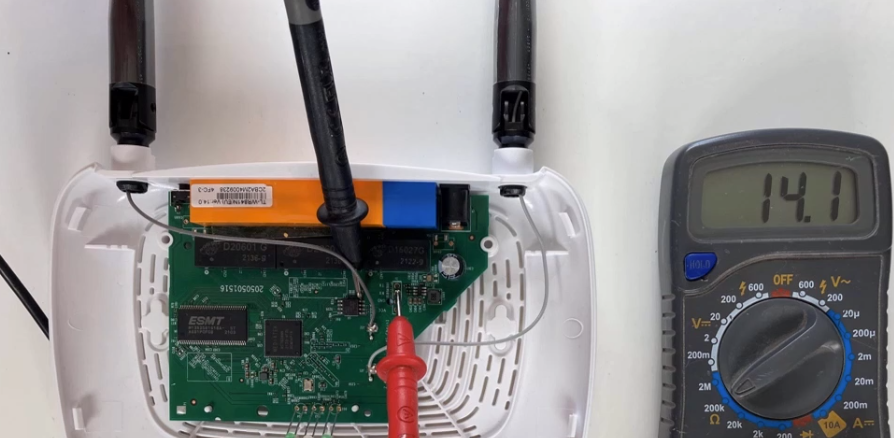
\includegraphics[scale=.4]{imagenes/1_UART_vcc.png}
     \label{fig:interfazUARTmedicionesvcc}
\end{figure}

After moving the red probe from pin 1 to pin 4, we obtain the following resistance values:

\begin{table}[htpb]
\centering
\caption{UART Electrical Measurements: GND and VCC}
\label{tab:my-table}
\begin{tabular}{@{}cccc@{}}
\toprule
{\color[HTML]{FE0000} \textbf{Pin}} & {\color[HTML]{FE0000} \textbf{R$_{GND}$}}                 & {\color[HTML]{FE0000} \textbf{R$_{VCC}$}}                 & {\color[HTML]{FE0000} \textbf{V}} \\ \midrule
\multicolumn{1}{|c|}{\textbf{1}}    & \multicolumn{1}{c|}{4.5 k$\Omega$}                        & \multicolumn{1}{c|}{14.1 k$\Omega$}                       &                                   \\ \midrule
\multicolumn{1}{|c|}{\textbf{2}}    & \multicolumn{1}{c|}{0.9 k$\Omega$}                        & \multicolumn{1}{c|}{11.0 k$\Omega$}                       &                                   \\ \midrule
\multicolumn{1}{|c|}{\textbf{3}}    & \multicolumn{1}{c|}{{\color[HTML]{FE0000} 0.0 k$\Omega$}} & \multicolumn{1}{c|}{10.0 k$\Omega$}                       &                                   \\ \midrule
\multicolumn{1}{|c|}{\textbf{4}}    & \multicolumn{1}{c|}{21.6 k$\Omega$}                       & \multicolumn{1}{c|}{{\color[HTML]{FE0000} 0.0 k$\Omega$}} &                                   \\ \bottomrule
\end{tabular}
\end{table}

\begin{tcolorbox}[enhanced, title=WARNING, colback=red!10]
For the final set of measurements, \textbf{\textcolor{red}{we now need to connect power to the router}}. We place the black probe again on the known ground reference. Be careful: now that power is connected, the router will show activity on the TX and RX pins. Which is TX and which is RX?
\end{tcolorbox}

Once the black probe is on GND and the system is powered, we know there will be activity between the flash chip (firmware) and SDRAM as it loads. To locate which pin is active, we use the red probe to measure the voltage from pin 1 to pin 4. The readings are:

\begin{table}[htpb]
\centering
\caption{UART Electrical Measurements: GND, VCC, and TX RX}
\label{tab:my-table}
\begin{tabular}{@{}cccc@{}}
\toprule
{\color[HTML]{FE0000} \textbf{Pin}} & {\color[HTML]{FE0000} \textbf{R$_{GND}$}}                 & {\color[HTML]{FE0000} \textbf{R$_{VCC}$}}                 & {\color[HTML]{FE0000} \textbf{V}} \\ \midrule
\multicolumn{1}{|c|}{\textbf{1}}    & \multicolumn{1}{c|}{4.5 k$\Omega$}                        & \multicolumn{1}{c|}{14.1 k$\Omega$}                       & \multicolumn{1}{c|}{3.25 V}       \\ \midrule
\multicolumn{1}{|c|}{\textbf{2}}    & \multicolumn{1}{c|}{0.9 k$\Omega$}                        & \multicolumn{1}{c|}{11.0 k$\Omega$}                       & \multicolumn{1}{c|}{0.0 V}        \\ \midrule
\multicolumn{1}{|c|}{\textbf{3}}    & \multicolumn{1}{c|}{{\color[HTML]{FE0000} 0.0 k$\Omega$}} & \multicolumn{1}{c|}{10.0 k$\Omega$}                       & \multicolumn{1}{c|}{0.0 V}        \\ \midrule
\multicolumn{1}{|c|}{\textbf{4}}    & \multicolumn{1}{c|}{21.6 k$\Omega$}                       & \multicolumn{1}{c|}{{\color[HTML]{FE0000} 0.0 k$\Omega$}} & \multicolumn{1}{c|}{3.3 V}        \\ \bottomrule
\end{tabular}
\end{table}

Pin 1 has shown resistance values relative to both GND and VCC, so it must be either TX or RX. We also noticed that when power was connected, this pin reached a voltage value of 3.3 volts. And clearly, nothing is being sent to the device. Therefore, we can conclude that PIN 1 is the TX PIN. If we monitor this pin (with an analog monitor) while powering the router, we will see voltage fluctuations, confirming that the router is sending data to the TX pin.

Just like PIN 1, PIN 2 shows resistance between GND and VCC. Since the measured voltage after powering the system is zero, it seems likely that this pin is RX, as nothing is being sent to the router.

PIN 3 is GND because there was no resistance to ground (and also no voltage when the router was powered), and PIN 4 is VCC because it showed zero resistance to VCC.

\begin{table}[htpb]
\centering
\caption{UART Electrical Measurements: Pin Identity}
\label{tab:my-table}
\begin{tabular}{@{}ccccc@{}}
\toprule
{\color[HTML]{FE0000} \textbf{Pin}} & {\color[HTML]{FE0000} \textbf{R$_{GND}$}}                 & {\color[HTML]{FE0000} \textbf{R$_{VCC}$}}                 & {\color[HTML]{FE0000} \textbf{V}} & \multicolumn{1}{l}{{\color[HTML]{3166FF} \textbf{Identity}}} \\ \midrule
\multicolumn{1}{|c|}{\textbf{1}}    & \multicolumn{1}{c|}{4.5 k$\Omega$}                        & \multicolumn{1}{c|}{14.1 k$\Omega$}                       & \multicolumn{1}{c|}{3.25 v}       & \multicolumn{1}{c|}{TX}                                       \\ \midrule
\multicolumn{1}{|c|}{\textbf{2}}    & \multicolumn{1}{c|}{0.9 k$\Omega$}                        & \multicolumn{1}{c|}{11.0 k$\Omega$}                       & \multicolumn{1}{c|}{0.0 v}        & \multicolumn{1}{c|}{RX}                                       \\ \midrule
\multicolumn{1}{|c|}{\textbf{3}}    & \multicolumn{1}{c|}{{\color[HTML]{FE0000} 0.0 k$\Omega$}} & \multicolumn{1}{c|}{10.0 k$\Omega$}                       & \multicolumn{1}{c|}{0.0 v}        & \multicolumn{1}{c|}{GND}                                      \\ \midrule
\multicolumn{1}{|c|}{\textbf{4}}    & \multicolumn{1}{c|}{21.6 k$\Omega$}                       & \multicolumn{1}{c|}{{\color[HTML]{FE0000} 0.0 k$\Omega$}} & \multicolumn{1}{c|}{3.3 v}        & \multicolumn{1}{c|}{VCC}                                      \\ \bottomrule
\end{tabular}
\end{table}

\section{Accessing the Firmware}

As previously described, firmware is software that is \emph{engraved} into the hardware. It is capable of operating without APIs, an operating system, or drivers. It provides the instructions and guidance necessary for the device to operate correctly, communicate with other drivers, and perform basic tasks.

Being able to extract the firmware from a device gives us the opportunity to identify weaknesses and vulnerabilities that could be exploited through traditional attack vectors, such as web attacks or network protocols. More critically, firmware stores information about device configuration and potentially sensitive data like passwords and encryption keys.

\subsection{The Path of Least Resistance}

An attacker will always choose the fastest and easiest path to access a system. Therefore, we must identify those paths. So, to analyze the firmware in this router, one could consider downloading it from the internet instead of illegally accessing the device to extract it.

Is it necessary to extract the firmware? Why not download it from the internet, analyze it, reveal the vulnerabilities, and exploit them to attack the device? And indeed, this would be the logical step if we couldn’t gain access to the router. Manufacturers provide access to firmware online primarily for updating the device.

Sometimes, downloading the firmware is useful because new versions \textbf{fix vulnerabilities found in previous versions}. If we identify vulnerabilities and match them to devices using those older firmware versions, \emph{voilà}, we have a ready-made attack vector.

We could also obtain the firmware through debugging ports, although this is a tedious and costly task. This would involve interrupting the boot process and interfacing with the \emph{bootloader} to execute commands that dump the firmware from memory to the screen, capturing the output through console logs.

But remember, information is transferred bit by bit:

\begin{verbatim}
    MATH TELLS US NOT TO DO IT:
    ---------------------------
    Flash memory size: 128 Mb
    Firmware is dumped via a serial link in hexadecimal.
    --> 1 byte = 2 hex characters + 1 space
    Each 2KB page adds 64 bytes for error correction.
    --> 3% overhead in code.
    A 128 MB chip = 128 x 3 x 1.03 = ~400MB
    Serial link speed = 115,200 kbps = 0.011 Mb/s.
    TOTAL TIME TO DUMP FIRMWARE: 9.6 hours
\end{verbatim}

So, dumping firmware through a serial link would take approximately \textbf{\textcolor{red}{10 hours}}, and we still wouldn’t be done. We would have a hex file that we’d need to convert to binary, trimming all unnecessary strings. This is a method to be used only when no other is available.

The next method would be to access the flash memory chip directly and dump its contents. To do this, we can connect the CH341A programmer to the memory chip using a SOIC clip. Once connected, we run the \textbf{flashrom} software (or similar) to extract the firmware directly from memory.

Another method is to try connecting to the device via TFTP and attempt to get a memory dump that way. This would require interrupting the router’s boot process to access the \emph{bootloader}, and we’d also need a TFTP server connected on the same subnet. For this to work, the device must have TFTP enabled—but this is very common, as TFTP servers are used for firmware updates, so the device likely already has one.

If none of these methods work, other options exist. For example, IoT devices occasionally broadcast a beacon to update servers to check (or request) updates. In that case, using Wireshark (or tcpdump), we can capture the update packets.

\subsection{Connection via UART}

The UART serial interface connection scheme for the router connects the router’s TX pin to the RX pin of the FT232. The FT232’s TX pin to the router’s RX pin. And the router’s GND pin to the FT232’s GND pin.

\begin{figure}[htpb]
     \caption{Firmware extraction via UART interface.}
     \centering
     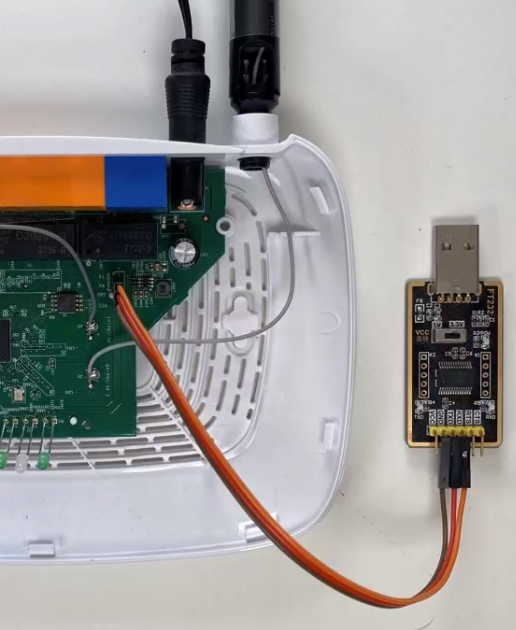
\includegraphics[scale=.4]{imagenes/2_Extraccion_UART.png}
     \label{fig:extraccionUART}
\end{figure}

From Fedora (as in my case) or from Windows, launch PuTTY.

\begin{figure}[htpb]
     \caption{Firmware extraction via UART interface.}
     \centering
     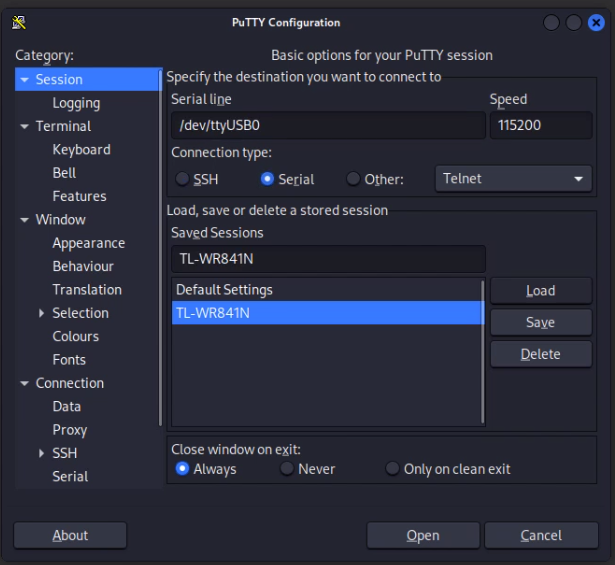
\includegraphics[scale=.4]{imagenes/2_PuTTY.png}
     \label{fig:PuTTY}
\end{figure}

As shown in Figure~\ref{fig:PuTTY}, the connection parameters (in this case, serial) must be configured. The device (on Linux) where the FT232 is mapped is \textbf{\textcolor{red}{/dev/ttyUSB0}}, and the transmission speed is 115200 kbps (UART speed on the router). In PuTTY’s Session section, under Logging, configure the following:

\begin{itemize}
    \item All session output.
    \item In "Log file name," specify the name of the log file to save the session.
    \item Always overwrite it.
    \item Flush log file frequently.
    \item Include header.
    \item Omit known password fields.
\end{itemize}

After this, PuTTY will be waiting for data from the router’s UART. Once we power it on, we’ll see the full router boot process (Figure~\ref{fig:UBOOT}):

\begin{figure}[htpb]
     \caption{Router boot process via U-BOOT.}
     \centering
     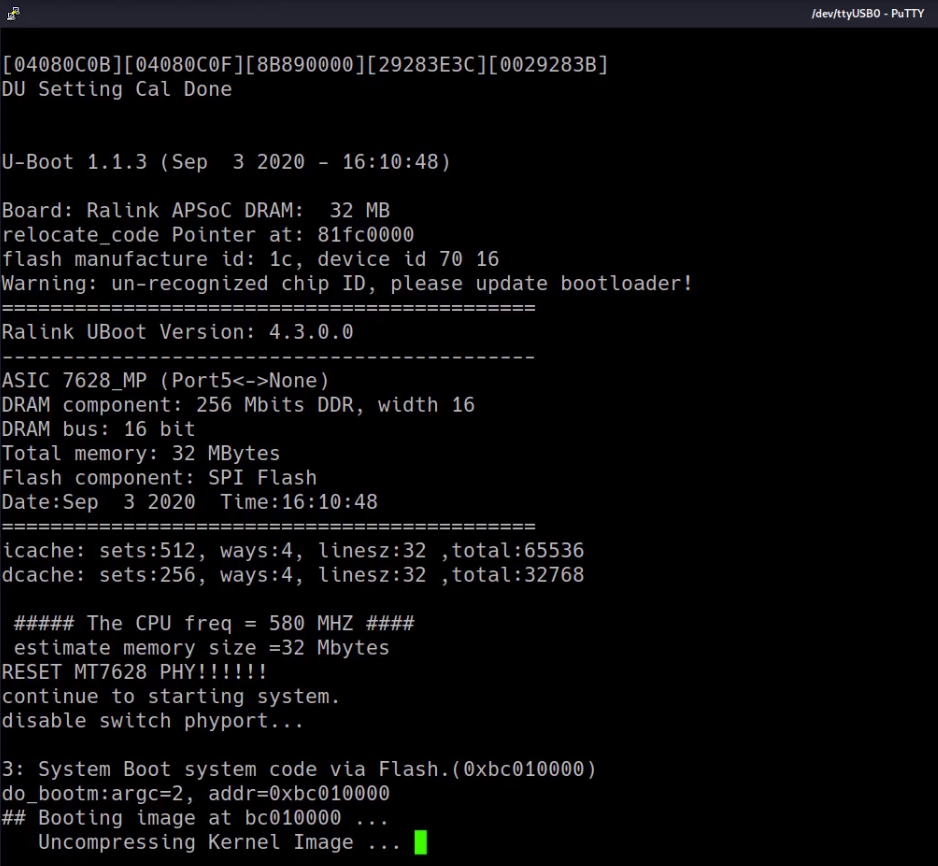
\includegraphics[scale=.4]{imagenes/2_UBOOT.png}
     \label{fig:UBOOT}
\end{figure}

There is a lot of interesting and useful information in these U-BOOT messages, which we can review in our log file. This data is useful as it reveals the memory organization and the location of \emph{file systems} in memory.

Once the router boot process completes, we get a prompt via the serial console. At boot, there is a process that floods the log with debug info. I’ve identified the process and, as soon as we get the prompt, I instruct the system to terminate it. The process has PID=\emph{174}, and the proper command to prevent this debug process from cluttering the log is: \emph{\textcolor{red}{kill -9 174}} (see Figure~\ref{fig:terminalRouter}). What we see through this interface is very similar to what we’d see on a standard Linux terminal:

\begin{figure}[htpb]
     \caption{Router console accessed via serial interface.}
     \centering
     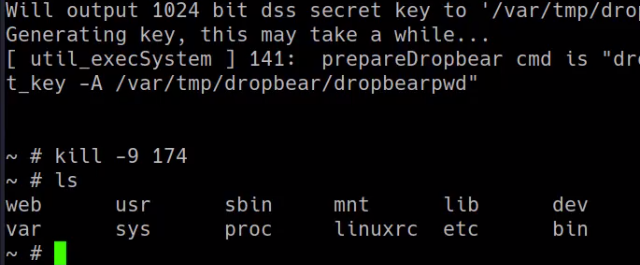
\includegraphics[scale=.6]{imagenes/2_terminalRouter.png}
     \label{fig:terminalRouter}
\end{figure}

If we list the contents of the \emph{/bin} directory (\emph{ls /bin}), we’ll find \underline{busybox}, giving us access to many more commands than the router shell normally provides. As shown in Figure~\ref{fig:TFTP}, we have access to the TFTP command.

\begin{figure}[htpb]
     \caption{Among other commands, busybox includes TFTP.}
     \centering
     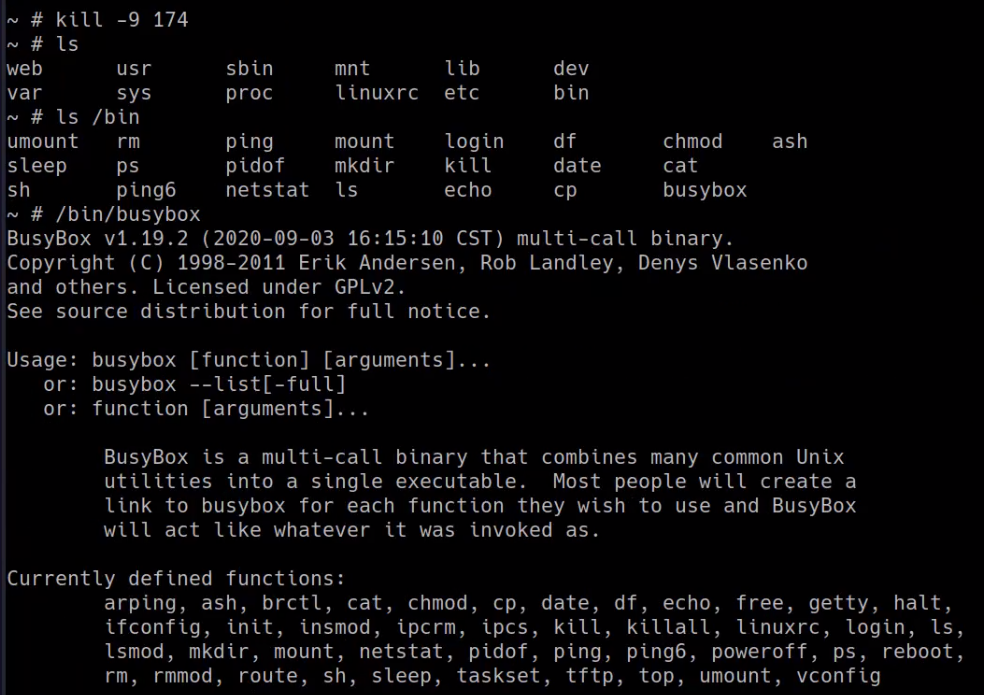
\includegraphics[scale=.4]{imagenes/2_tftp.png}
     \label{fig:TFTP}
\end{figure}
However, this is not a full busybox installation. If we check the /sbin directory (which can only be accessed with superuser privileges or if you belong to the wheel group), we can see which commands are available:

\begin{figure}[htpb]
     \caption{Contents of /sbin and /etc. Listing of the /etc/passwd file}
     \centering
     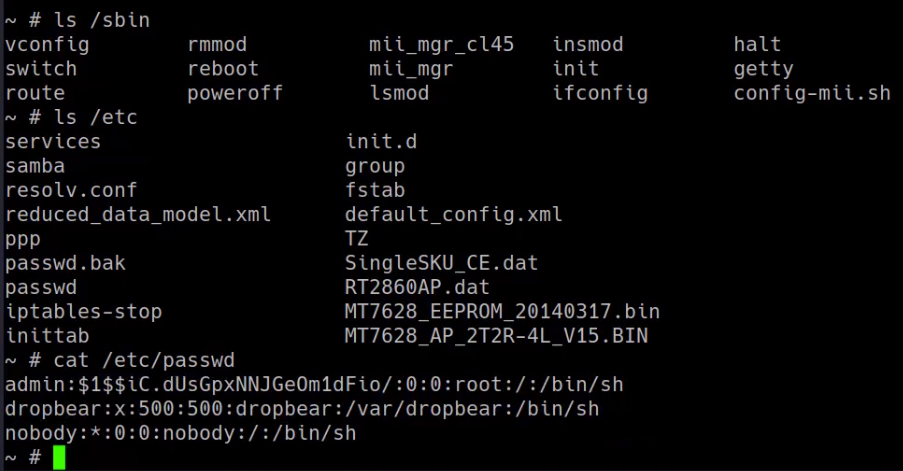
\includegraphics[scale=.4]{imagenes/2_etcsbin.png}
     \label{fig:etcsbin}
\end{figure}

Figure~\ref{fig:etcsbin} shows both the /sbin and /etc directories. In the /etc directory, we find the password file (specifically the file with \emph{password hashes}), which is interesting for determining which users are configured on the router. For the user \textbf{admin}, we can see the hash (which encodes the password), and we could use \textbf{hashcat} to try to crack the hash and obtain the admin credentials. However, since the router is ours, that wouldn’t make sense. What’s useful here is knowing which users exist so we can assess what functionality may be exploitable.

Looking into the /lib directory is interesting as well because we can see which functionality is shared. A \emph{.so} file is a shared library that resides in a memory area and is shared by programs that require its functionality, instead of incorporating the library into each program’s address space. That way, we can investigate the shared libraries used by the router’s programs and analyze whether they have any known vulnerabilities that could be exploited to attack the processes relying on that library.

\begin{figure}[htpb]
     \caption{Contents of /lib}
     \centering
     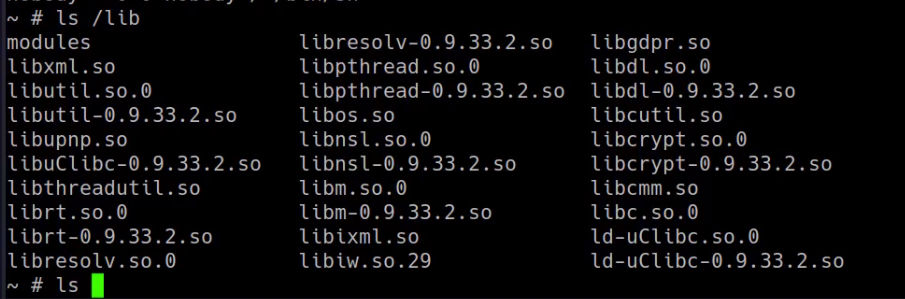
\includegraphics[scale=.4]{imagenes/2_lib.png}
     \label{fig:lib}
\end{figure}

Thus, the next (almost) logical step is to see which processes are running on the router. We do this by executing \emph{ps}, which gives us very useful information:

\begin{figure}[htpb]
     \caption{Running processes: interesting to see httpd and dropbear.}
     \centering
     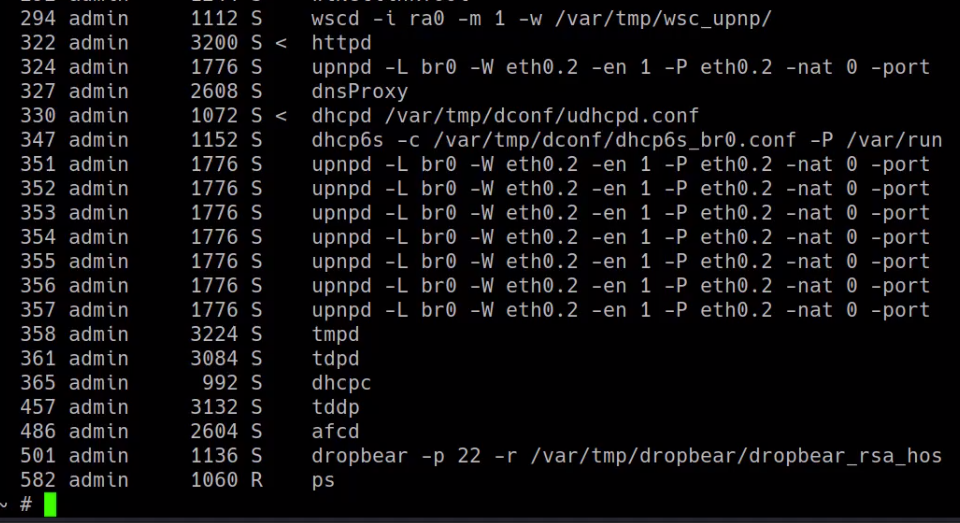
\includegraphics[scale=.4]{imagenes/2_httpdssh.png}
     \label{fig:httpddropbear}
\end{figure}

We see that the router has the \textcolor{red}{SSH server dropbear} running on port \textcolor{red}{22}, and we also have an \textcolor{red}{HTTP daemon}, meaning there's a web server on the router. This web server is used to provide the user with a configuration interface. Figure~\ref{fig:netstat} shows how, using the \emph{netstat} command, we can see the connections currently open on the router. Note that the router is not connected to the Internet.

\begin{figure}[htpb]
     \caption{Open connections (netstat).}
     \centering
     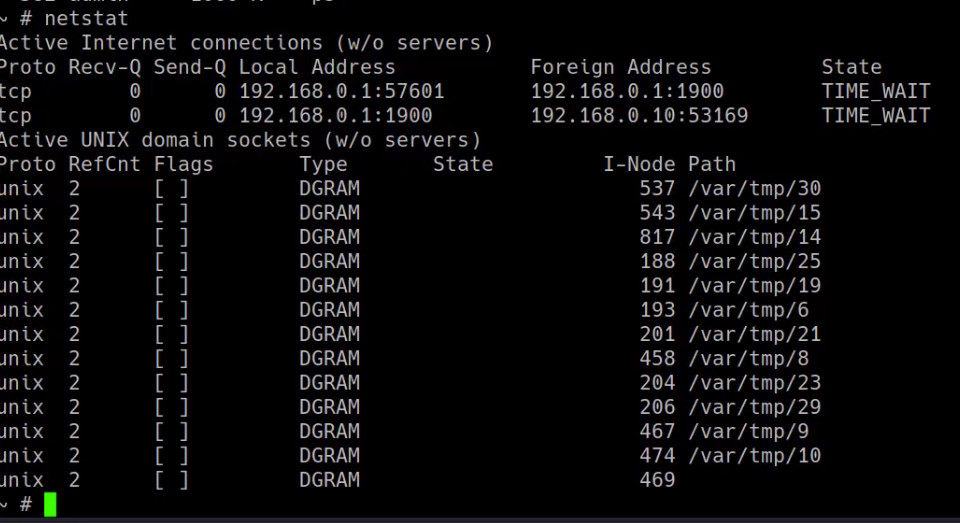
\includegraphics[scale=.4]{imagenes/2_netstat.png}
     \label{fig:netstat}
\end{figure}

In Figure~\ref{fig:netstat}, ports 21 (FTP) and 23 (TELNET) are particularly interesting and revealing. Our router opens those ports. Now that we have a rough idea of the router’s basic configuration, the next step is to check how far (i.e., what privileges) we can go. For that, we need to verify which user we are logged in as. Remember, from the /etc/passwd file we saw that there were three users. The command \emph{whoami} would tell us which user is currently active via UART. Unfortunately, we don’t have that command. We also don’t have \emph{uname}, which would let us see kernel details.

In this situation, we’re left with \emph{busybox} and TFTP. One option would be to extend the available commands using TFTP to download a more advanced and complete version of busybox. With more commands available, we can extract more information. However, we should first check the file system to see where we are allowed to write (i.e., where to download things). To do this, we use the \emph{mount} command. This shows us that the only writable part of the file system (yes, to download a full busybox) is /var.

\begin{figure}[htpb]
     \caption{Where can we deploy (write) files?}
     \centering
     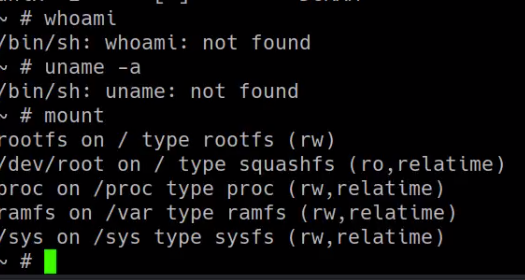
\includegraphics[scale=.4]{imagenes/2_var.png}
     \label{fig:var}
\end{figure}

\begin{tcolorbox}[colback=red!10, title=We Set Up Our TFTP Server]
We need to prepare our \textbf{payload}. In this case, it will be a version of busybox for MIPS (\emph{busybox-mipsel}). We must download the file from this web server: \href{https://busybox.net/downloads/binaries/1.16.1/}{https://busybox.net/downloads/binaries/1.16.1/} and select the \emph{busybox-mipsel} file.

The steps followed are:

\begin{itemize}
    \item \textbf{SUBNET:} Connect the laptop to the router so that they are on the same subnet (my laptop gets the IP address 192.168.0.10).
    \item \textbf{TFTP:} Install a TFTP server and place the downloaded file in the root directory so we can fetch the more powerful busybox.
    \item \textbf{Connecting from the router to the server:} We want to download \emph{busybox-mipsel} into the /var directory of the router. To do that, on the router we execute:
    \begin{itemize}
        \item \textbf{cd /var} (to access /var, the only writable directory).
        \item \textbf{tftp -g -r busybox-mipsel 192.168.0.10} (parameters used: g = get, r = remote).
    \end{itemize}
    \item \textbf{Downloaded:} We need to make it executable by running \textbf{chmod +x busybox-mipsel}.
\end{itemize}
\end{tcolorbox}

Once we have \emph{busybox-mipsel} inside the router, we can run it using \emph{./busybox-mipsel} (from the /var directory, where we downloaded it, of course). Then we can observe three things (see Figure~\ref{fig:busyboxgrande}):

\begin{itemize}
    \item When executing \emph{./busybox-mipsel}, we see that the number of available commands is much greater than with the default busybox on the router.
    \item We can now run \textbf{whoami} to see which user is assigned. The user is \textbf{admin}.
    \item We can now view kernel details (2.6.36) on a MIPS architecture. It is surprising that a router purchased in 2023 uses a 2010 kernel. Being so old, there are likely several vulnerabilities we can exploit.
\end{itemize}

\begin{figure}[htpb]
     \caption{Busybox-mipsel: access to more commands.}
     \centering
     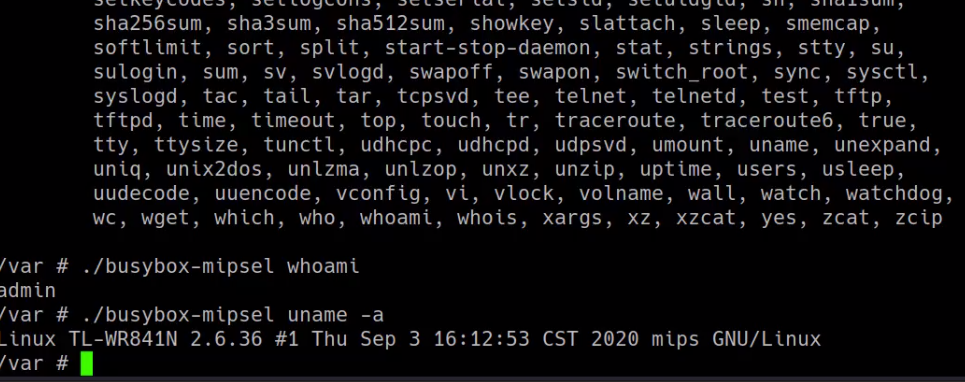
\includegraphics[scale=.4]{imagenes/2_busyboxgrande.png}
     \label{fig:busyboxgrande}
\end{figure}

At this point, I’ve discovered that the router (when accessed via the serial interface (UART)) grants administrator access. So the hardest part is essentially done—we have \emph{root} access to the device. Now we need to use this access to extract the firmware from the device.

\subsubsection{Firmware Extraction via UART}

If we check the log, we can see that during the router’s boot process, five MTD (Memory Technology Device) partitions are created. These are used in Linux to interact with flash memory (where the firmware is stored). This subsystem was created to act as an intermediary (an abstraction layer) between hardware-specific drivers and higher-level applications.

\begin{figure}[htpb]
     \caption{MTD (Memory Technology Device) partitions.}
     \centering
     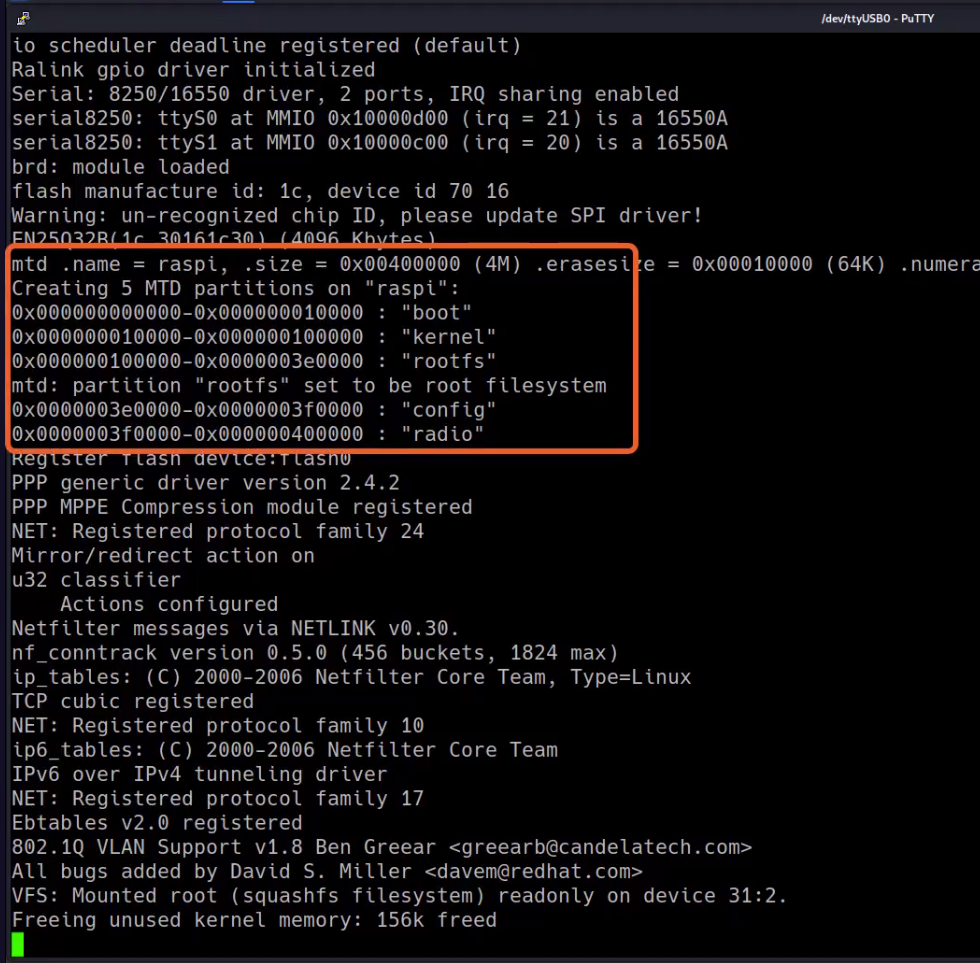
\includegraphics[scale=.4]{imagenes/2_mtd.png}
     \label{fig:mtd}
\end{figure}

Once we’re inside the router, we can see MTD partition information within the virtual file system in /proc. This MTD subsystem is mounted inside the /dev directory (devices).

\begin{figure}[htpb]
     \caption{MTD (Memory Technology Device) partitions in /proc.}
     \centering
     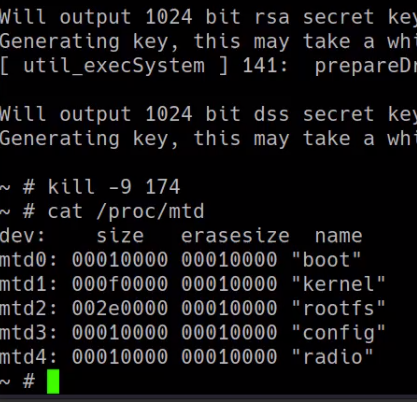
\includegraphics[scale=.6]{imagenes/2_procMTD.png}
     \label{fig:procmtd}
\end{figure}
So if we list the contents of the /dev directory (\emph{ls -al /dev}):

\begin{figure}[htpb]
     \caption{MTD (Memory Technology Device) partitions in /dev.}
     \centering
     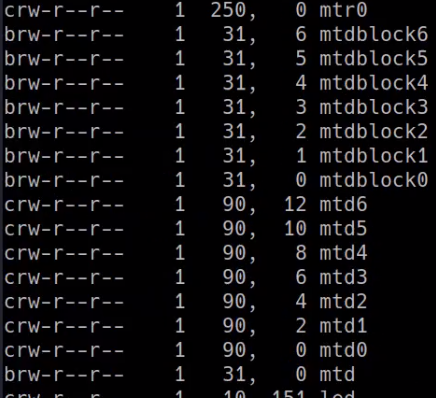
\includegraphics[scale=.6]{imagenes/2_devmtd.png}
     \label{fig:devmtf}
\end{figure}

If we observe the permissions, we can see that MTD blocks from zero to six are block devices\footnote{They are non-volatile mass storage devices whose information can be accessed randomly. More specifically, an MTD block is used to present flash memory as a block device that can be formatted and mounted as part of the file system.}. If we inspect one of these devices (\emph{cat /dev/mtdblock0}), we will see a mix of characters, some readable and others unreadable.

\begin{figure}[htpb]
     \caption{Content (characters) of an mtd block.}
     \centering
     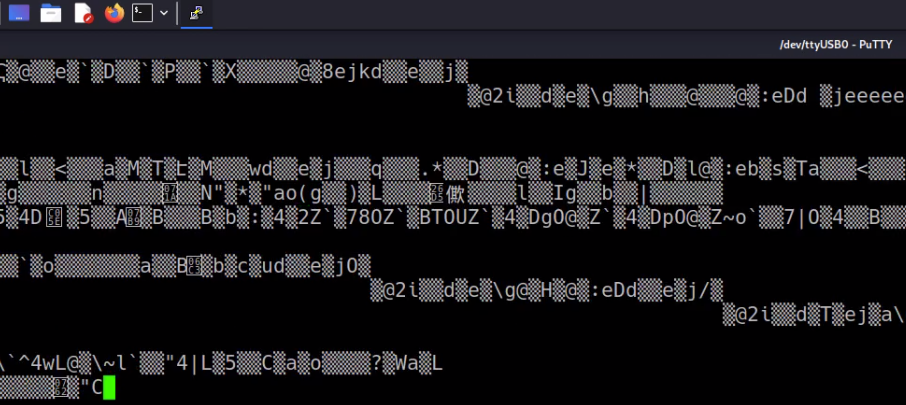
\includegraphics[scale=.4]{imagenes/2_garbage.png}
     \label{fig:garbage}
\end{figure}

This is exactly what we would expect to find, just like when opening a disk or USB drive with an ASCII editor. Therefore, if we want to \emph{access the content of the MTDs}, we can do so using \emph{cat} and save the output to then analyze it with \emph{binwalk}. Instead of doing this manually, we will use the following Python script, which connects via serial and extracts the content of each MTD.

\begin{tcolorbox}[colback=blue!10, title=Script to access MTD contents: extraccion\_via\_uart.py]
\begin{verbatim}
import serial
import time

port = serial.Serial("/dev/ttyUSB0", baudrate=115200, timeout=60.0)
port.write("\n".encode())
time.sleep(1)

while True:
    port.flush()
    time.sleep(1)
    f = open("rootfs_via_uart.img", "w")
    f.write('')
    f.close()
    f = open("rootfs_via_uart.img", "a")
    port.write("cat /dev/mtdblock2\n".encode())

    buffer = ''
    contador = 0
    while True:
        time.sleep(0.001)
        bytesporleer = port.inWaiting()
        time.sleep(0.001)
        contador = contador + 1
        if bytesporleer > 0: 
            contador = 0
            print ("Bytes to read: " + str(bytesporleer))
            buffer = port.read(bytesporleer)
            print ("Read: " + str(buffer))
            f.write(buffer.decode(encoding='latin-1'))
            time.sleep(0.001)
        if contador > 1000:
            if f.tell() > 2000000:
                print ("Done")
                while True:
                    pass
            print ("Error! Size: " + str(f.tell()) + " Bytes")
            port.write("\x03".encode())
            time.sleep(1)
            break
\end{verbatim}
\end{tcolorbox}

If we launch the Python script from the Linux terminal (or Windows console): \emph{python extraccion\_via\_uart.py}, we will see output on the screen (because we’ve included it in the script; we could remove this to speed it up):

\begin{figure}[htpb]
     \caption{Download of 496 bytes per iteration via UART.}
     \centering
     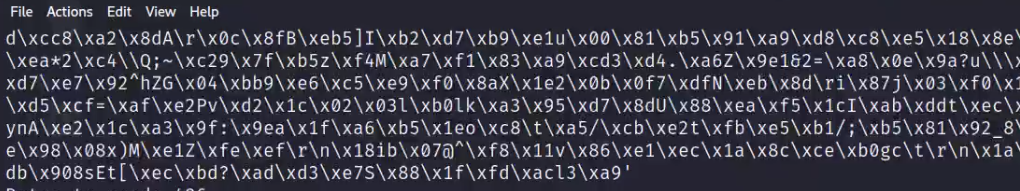
\includegraphics[scale=.4]{imagenes/2_dump.png}
     \label{fig:dump}
\end{figure}

Downloading this file took almost half an hour. Before analyzing this binary with \textbf{binwalk}, we must clean it by removing unnecessary strings and converting hexadecimal to binary. For this, any hex-to-binary conversion tool will work. When running \emph{binwalk rootfs\_via\_uart.img}, we find a \textbf{squash} file system of 3 MB.

\begin{figure}[htpb]
     \caption{Binwalk on the downloaded file.}
     \centering
     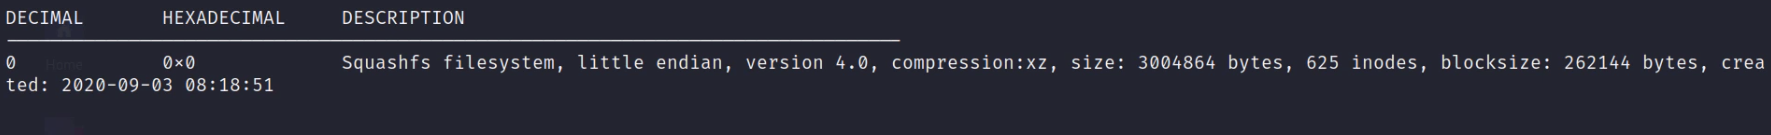
\includegraphics[scale=.28]{imagenes/2_binwalk.png}
     \label{fig:binwalk}
\end{figure}

\subsection{Extraction via Flash Memory Dump}

What if we can’t access a console (terminal) that gives us command line access to the router? Then we must extract the firmware by directly targeting the chip that holds it—that is, the flash memory chip—using the CH341A programmer and the \textbf{flashrom} application. As before, we will verify the extracted data using \emph{binwalk}.

\begin{figure}[htpb]
     \caption{Direct extraction from the chip using a SOIC clip and CH341A programmer.}
     \centering
     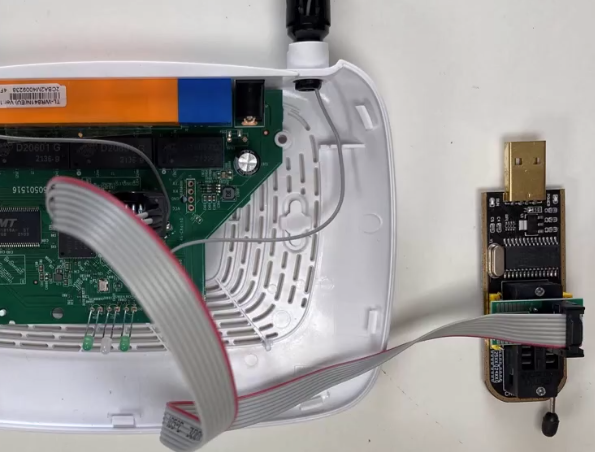
\includegraphics[scale=.5]{imagenes/2_ch341A.png}
     \label{fig:ch341a}
\end{figure}

On the SOIC clip, the red wire must be connected to pin 1 of the chip. Pin 1 is usually marked on the chip. Connecting it can be tricky, as the clip may loosen, and we must ensure it is properly reattached. If a non-SOIC clip is used, only the SPI communication pins may be needed (in this chip: pins 1, 2, 4, 5, and 6). You should always check the datasheet to confirm which pins to use. On this chip, pins 1 to 4 are on one side (pin 1 marked), and pins 5 to 8 are on the opposite side.

\begin{tcolorbox}[colback=red!10, title=Attention]
To extract firmware from the flash memory chip, do \textbf{not} power the device, as doing so would start the boot process, and the chip we're working with is the one that initiates it.
\end{tcolorbox}

\begin{tcolorbox}[colback=green!10, title=Using flashrom to read the flash memory chip]
\textbf{flashrom --programmer ch341a\_spi -r TL-WR841N\_firmware.bin}

In this case, we are using a generic CH341A programmer. The \texttt{-r} option instructs flashrom to read the flash and save the output to the file we specify.

It is common for flashrom to request elevated privileges, but in our case, it is unnecessary because we are using a USB programmer supported by flashrom.
\end{tcolorbox}

When executing flashrom, it quickly detects the memory chip. This method took less than 40 seconds to extract the entire flash memory contents.

\begin{figure}[htpb]
     \caption{Flashrom.}
     \centering
     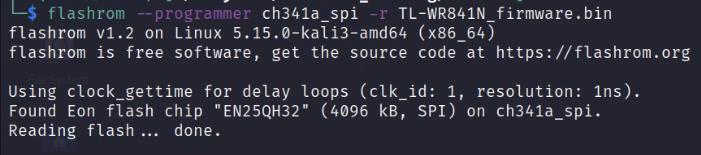
\includegraphics[scale=.7]{imagenes/2_flashrom1.png}
     \label{fig:flashrom1}
\end{figure}

In this case, unlike the UART extraction, there is no need to preprocess the binary file because we extracted it bit by bit directly from its source. It’s a faster and less tedious method. After downloading the firmware, we always analyze it with \textbf{binwalk} to check if the image was properly generated.

\begin{figure}[htpb]
     \caption{Binary extracted from flash chip analyzed with binwalk}
     \centering
     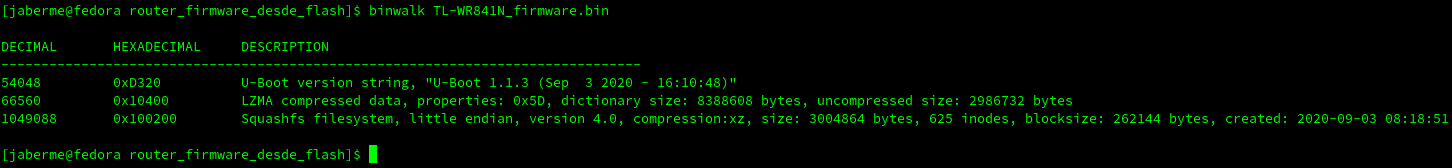
\includegraphics[scale=.35]{imagenes/2_flash.png}
     \label{fig:flash}
\end{figure}

We can immediately identify the U-BOOT loader, LZMA-compressed data, and a \emph{SquashFS} file system. So it seems we’ve once again successfully obtained the image.

\subsection{Extraction via TFTP Directly from RAM}

In this method, we access the file system from the MTD. But instead of extracting it through a slow serial connection (like UART), we will do so via TFTP, which we already installed when we placed \emph{busybox-mipsel} in the /var directory.

What we need to set up again is our small TFTP server, which will receive the firmware. So we reconnect the FT232 to the UART pins, just like we did in the UART section. This gives us console access (router terminal) again, and we will initiate an FTP connection from the router to our TFTP server and send it the firmware. This time we connect the router and our laptop using an Ethernet cable, configuring both on the same subnet.

Since we’ll access RAM, which is represented by the MTD block devices (see Figure~\ref{fig:mtd}), we must remember that there are five partitions created when the router reboots. Their presence was previously verified using the \emph{cat /proc/mtd} command, as seen in Figure~\ref{fig:procmtd}. We can extract each of those partitions, but the most important one is the \textbf{rootfs} partition.

\begin{figure}[htpb]
     \caption{Firmware transfer via TFTP}
     \centering
     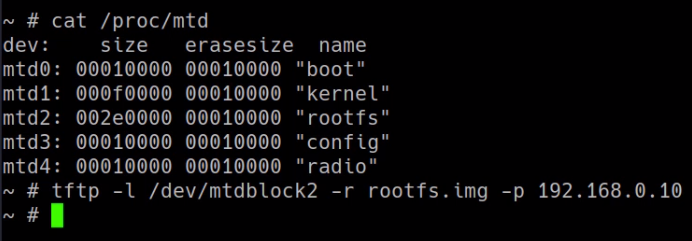
\includegraphics[scale=.35]{imagenes/2_tftpram.png}
     \label{fig:tftpram}
\end{figure}

In just a few seconds, we will have received the rootfs partition on our TFTP server.

\section{Firmware Analysis}

We now have in our possession a binary file—the firmware image of our target device. With it, we can perform several tasks, which we can group into two categories:

\begin{itemize}
    \item \textbf{Sensitive Information:} Identify sensitive data in the image, such as credentials, encryption keys, hashes, etc.
    \item \textbf{Vulnerability Research:} Determine what software the router has installed to look for weaknesses. These vulnerabilities might even affect the device’s operating system.
\end{itemize}

Before doing anything else, we need to identify and understand the structure of the image extracted from the router. Figure~\ref{fig:rom} shows the raw binary file extracted from the router. Since we’ll be working with it, we make a backup named \texttt{rom2.bin} to analyze and understand its structure. In this figure, we can see that \emph{binwalk} (the analysis command is simple: \emph{binwalk rom2.bin}) can interpret the internal structure of the binary file.
\begin{figure}[htpb]
     \caption{Images extracted from the router}
     \centering
     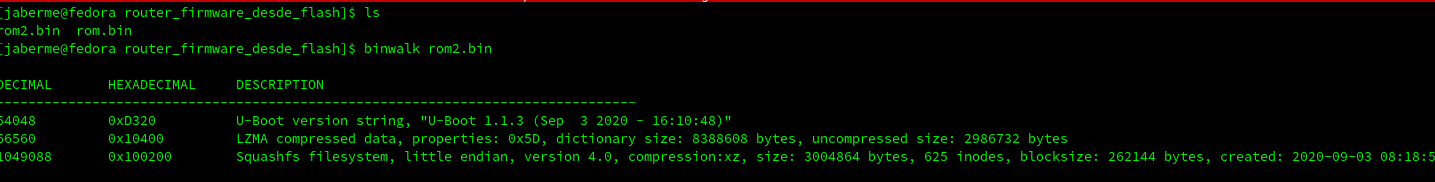
\includegraphics[scale=.35]{imagenes/rom.png}
     \label{fig:rom}
\end{figure}

The binary file we extracted contains:
\begin{itemize}
    \item The bootloader used by the router to start everything (load the OS image into memory):
    \begin{tcolorbox}[colback=red!10]
            \begin{verbatim}
U-Boot version string, "U-Boot 1.1.3 (Sep  3 2020 - 16:10:48)".
            \end{verbatim}
    \end{tcolorbox}
    We can see that the bootloader starts at byte 54048.
    
    \item Files compressed with LZMA:
    \begin{tcolorbox}[colback=red!10]
            \begin{verbatim}
LZMA compressed data.
            \end{verbatim}
    \end{tcolorbox}
    These data start at byte 66560.
    
    \item The complete file system of the router:
    \begin{tcolorbox}[colback=red!10]
            \begin{verbatim}
Squashfs filesystem, little endian, version 4.0.
            \end{verbatim}
    \end{tcolorbox}
    The file system starts at around 1 MB (byte 1049088).
\end{itemize}

Binwalk may sometimes give false positives or inaccurate information. For example, in the segment corresponding to compressed LZMA data, it tells us that the compressed dictionary occupies 8.3 MB, while the decompressed one is 2.9 MB. Besides this, binwalk allows us to analyze the binary’s \textbf{entropy}.

\begin{tcolorbox}[colback=green!10]
    \textbf{Entropy} is a concept inherited from other disciplines like thermodynamics or chemistry. It measures disorder—and therefore, irreversibility. In computer engineering, it is used to determine, for example, whether a segment of binary data is encrypted and therefore may (in certain contexts) contain malware. In a binary file, entropy measures the randomness of the data.
\end{tcolorbox}

Figure~\ref{fig:entropia} shows the randomness of the router firmware. The Y-axis shows entropy values (from 0 to 1). High entropy values (above 0.7) usually indicate that the data is \textbf{obfuscated\footnote{Obfuscation consists of adding meaningless data to useful data to hinder analysis.}}, especially when we know the file contains structured data and yet entropy is high. That likely means the useful data is being intentionally hidden (obfuscated).

\begin{figure}[htpb]
     \caption{Entropy of rom.bin}
     \centering
     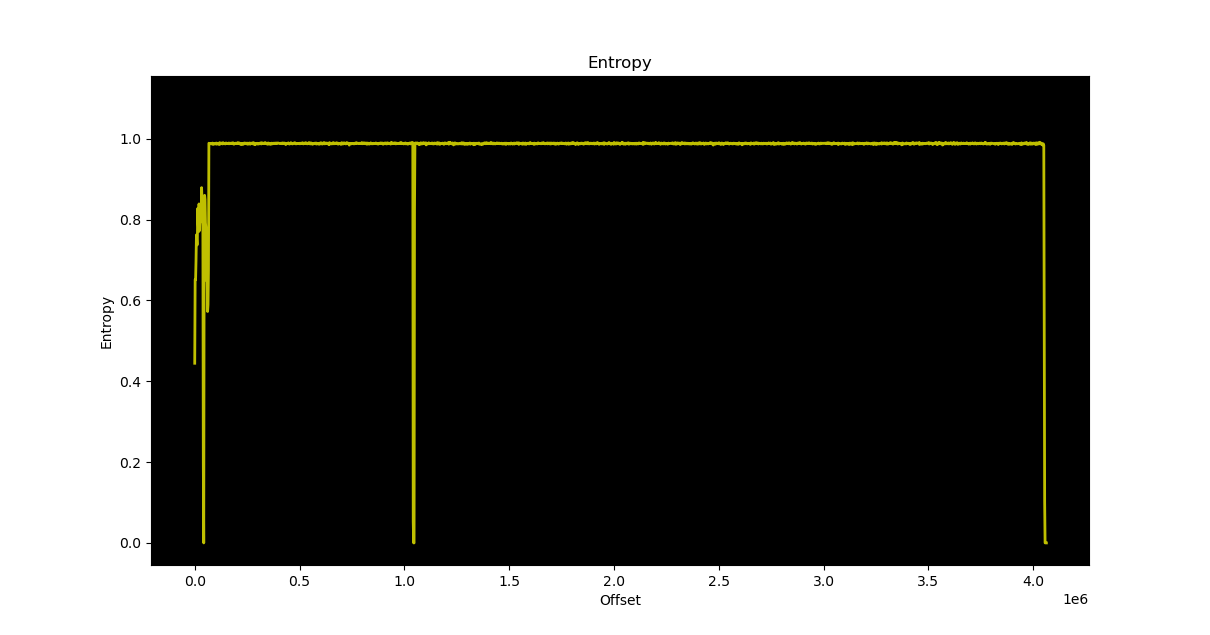
\includegraphics[scale=.6]{imagenes/entropia.png}
     \label{fig:entropia}
\end{figure}

Figure~\ref{fig:entropia} tells us that most of the file is obfuscated, except for a small portion at the beginning. Of the three parts that make up the binary file, the most interesting one for verifying the router’s security is the last—the one containing the \textbf{Squashfs} file system.

\begin{tcolorbox}[colback=green!10]
\textbf{Squashfs} is a Linux \textbf{compressed, read-only} file system. So it’s very likely that if we find a Squashfs on a device (like our router), it will contain the entire directory tree.
\end{tcolorbox}

\subsection{Analyzing the interesting part of the extracted binary}

We need to extract, from the binary file \texttt{rom.bin} (in our case, we keep a backup to preserve the original data), the segment corresponding to the Squashfs file system.

\begin{tcolorbox}[colback=green!10]
To extract information, we can use the capabilities of \textbf{binwalk}, although we will also see how to use the Linux command \textbf{dd}, which is useful when binwalk is unavailable. We can use the direct \texttt{-e} option: \textbf{\emph{binwalk -e rom2.bin}} to extract all the data. Alternatively, we can extract each binary segment with: \textbf{\emph{binwalk --dd='.*' rom2.bin}}
\end{tcolorbox}

Running \textbf{\emph{binwalk --dd='.*' rom2.bin}} produces (see Figure~\ref{fig:extraccion1}) several binary files, including the LZMA-compressed archive:

\begin{figure}[htpb]
     \caption{Extraction of binaries from rom.bin}
     \centering
     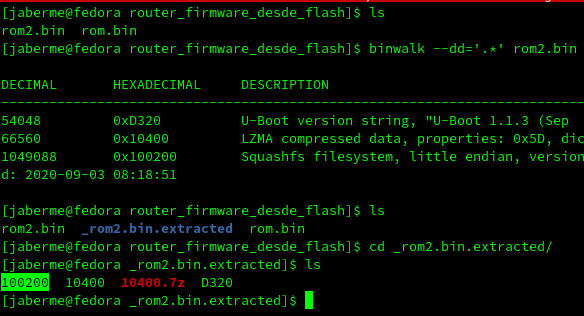
\includegraphics[scale=.6]{imagenes/extraccion1.png}
     \label{fig:extraccion1}
\end{figure}

If we look closely, one binary file is named with the hexadecimal offset (100200), which matches the start of the Squashfs file system. Analyzing that file again with binwalk shows that we now have the file system isolated:

\begin{figure}[htpb]
     \caption{Extraction of binaries from rom.bin}
     \centering
     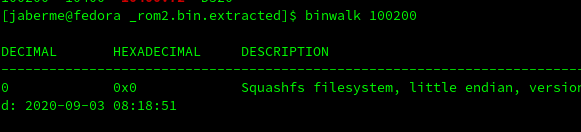
\includegraphics[scale=.6]{imagenes/extraccion2.png}
     \label{fig:extraccion2}
\end{figure}

Now we can extract the contents using \textbf{\emph{binwalk -e 100200}}. Could we have used \textbf{\emph{binwalk -e rom2.bin}} to extract everything (bootloader, LZMA, squashfs)? YES. But in this case, we chose to extract only the binary we care about from \texttt{rom2.bin}, and then extract the contents of that segment only—instead of unpacking all binaries from the main firmware file.

After extraction, a directory is created (in our case) named \textcolor{blue}{\textbf{\_100200.extracted}}, and inside it we find what really interests us: \textcolor{blue}{\textbf{squashfs-root}}.

\begin{figure}[htpb]
     \caption{squashfs}
     \centering
     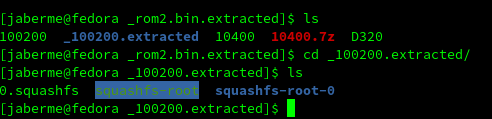
\includegraphics[scale=.6]{imagenes/squashfs-root.png}
     \label{fig:squashfs}
\end{figure}

If we access that directory, we gain access to the entire directory tree. Inside \texttt{/etc} (see figure) we find two very interesting files:

\begin{figure}[htpb]
     \caption{Interesting files in squashfs-root/etc}
     \centering
     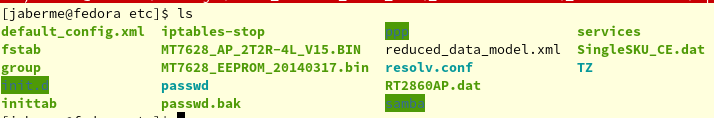
\includegraphics[scale=.6]{imagenes/passback.png}
     \label{fig:pass}
\end{figure}

\begin{itemize}
    \item \texttt{passwd.bak}: its contents match what we saw earlier:
    \begin{itemize}
        \item admin:\$1\$\$iC.dUsGpxNNJGeOm1dFio/:0:0:root:/:/bin/sh
        \item dropbear:x:500:500:dropbear:/var/dropbear:/bin/sh
        \item nobody:*:0:0:nobody:/:/bin/sh
    \end{itemize}

    \begin{tcolorbox}[colback=blue!10]
        \textbf{Users}: admin:\$1\$\$iC.dUsGpxNNJGeOm1dFio/:0:0:root:/:/bin/sh. \\
        \textbf{admin user's hash}: \$1\$\$iC.dUsGpxNNJGeOm1dFio/ \\
        There are tools like \textbf{hashcat} or \textbf{JohnTheRipper} that can be used to crack the hash and obtain the admin user's password.
    \end{tcolorbox}

    \item \texttt{default\_config} (this is an XML file)
\end{itemize}

\begin{tcolorbox}[colback=green!10]
    \textbf{dd}: Another way to extract the \emph{SquashFS} file system without using binwalk is to use the command: \\
    \texttt{dd if=rom2.bin skip=1049088 of=sistemaDeArchivos bs=1}, where:
    \begin{itemize}
        \item \texttt{if}: identifies the input file
        \item \texttt{skip}: number of bytes to skip in the input file
        \item \texttt{of}: output file (in this case we name it \texttt{sistemaDeArchivos})
        \item \texttt{bs}: block size; using 1 means skip 1049088 bytes exactly
    \end{itemize}
    The result is the file system stored in a single binary file. To extract it (without using binwalk), use: \\
    \texttt{unsquashfs sistemaDeArchivos}
\end{tcolorbox}

\subsubsection{Password cracking}

\begin{tcolorbox}[colback=red!10]
    \textbf{Password cracking or hash cracking} is the technique of discovering passwords based solely on their encoded hash. To do this, it's necessary to know the hashing algorithm and have a dictionary of potential password candidates. The simplest technique is brute force, which involves trying all possible letter and number combinations (once the algorithm is known), generating the hash, and checking for a match with the target hash. If a \emph{match} occurs, that combination is likely the correct password. The two most powerful tools for this are \textbf{JohnTheRipper} and \textbf{hashcat}. Hashcat was developed by Europol.
\end{tcolorbox}

Regardless of how we access the squashfs, we can extract the admin hash from the \texttt{/etc} directory and try to crack it using JohnTheRipper or hashcat. In our case, we didn’t even need \emph{hashcat}—we found the password quickly using JohnTheRipper’s default attack: \textbf{\textcolor{red}{john passwd.bak}}.
\begin{figure}[htpb]
     \caption{Password cracking}
     \centering
     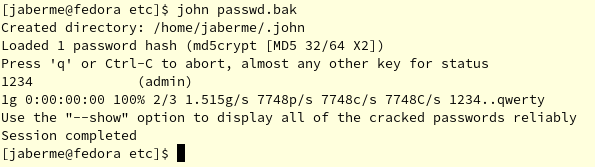
\includegraphics[scale=.8]{imagenes/john.png}
     \label{fig:pass}
\end{figure}

\begin{tcolorbox}[colback=red!5]
    In the case of this router, the hash was created using \textbf{MD5}, which is a very insecure hashing algorithm: \textbf{\textcolor{red}{first vulnerability}}.
\end{tcolorbox}

\subsubsection{Selective Extraction}

If we recall, the file containing the firmware (Figure~\ref{fig:rom}) indicated that we had a set of files compressed with LZMA, and this block of data lies between the bootloader and the file system (which we’ve already extracted and found to contain interesting information under the /etc directory, including the opportunity to practice password cracking). If we want to extract the LZMA-compressed data, we need to extract this binary segment from the \texttt{rom2.bin} file (our working copy of \texttt{rom.bin}, which we originally pulled from the router).

We know the LZMA segment begins at byte 66560 and continues until the start of the file system (1049088). Thus, the segment spans from byte 66560 to byte 1049088, meaning it occupies 1049088 - 66560 = 982528 bytes. This doesn’t mean all of those bytes hold data. We only know we need to extract 982528 bytes, and we already know how to do that with \texttt{dd}:

\begin{verbatim}
dd if=rom2.bin skip=66560 count=982528 of=archivoComprimido.lzma bs=1
\end{verbatim}

\texttt{count} indicates the number of bytes to extract starting from offset 66560.

Since we don’t know how many of those 982528 bytes contain actual data and how much is just padding, we can use the \texttt{lzma} command to clean out the useless portion:

\begin{verbatim}
lzma -d < archivoComprimido.lzma > archivoFinal
\end{verbatim}

The output from this command may indicate that the generated file (\texttt{archivoFinal}) is corrupted, but that’s not actually the case. In fact, if we analyze it with \texttt{binwalk}, it reveals all its content, including a segment labeled \textbf{xz compressed data} (which draws attention). Segments before that include the kernel version and CRC checks. Another relevant structure is the \texttt{ASCII cpio archive}, used for dumping and restoring backup data in readable ASCII encoding. Figure~\ref{fig:lzma} shows the commands and output from my terminal:

\begin{figure}[htpb]
     \caption{Extracting the other segment (LZMA)}
     \centering
     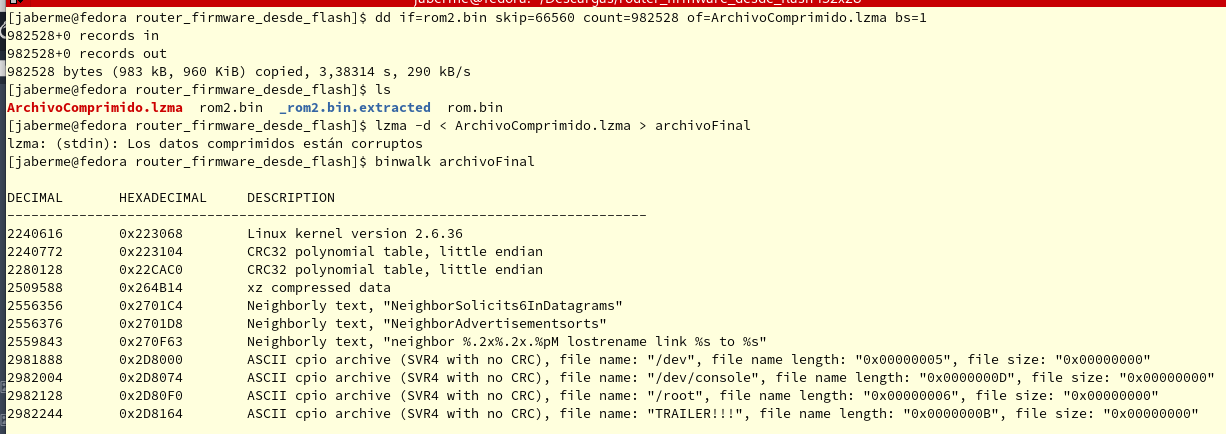
\includegraphics[scale=.38]{imagenes/lzma.png}
     \label{fig:lzma}
\end{figure}

If we analyze the entropy of this segment, we’ll see that at the end (where the ASCII-readable data resides), entropy is below 0.7, meaning this information is \textbf{not obfuscated}.

\begin{figure}[htpb]
     \caption{Entropy of archivoFinal}
     \centering
     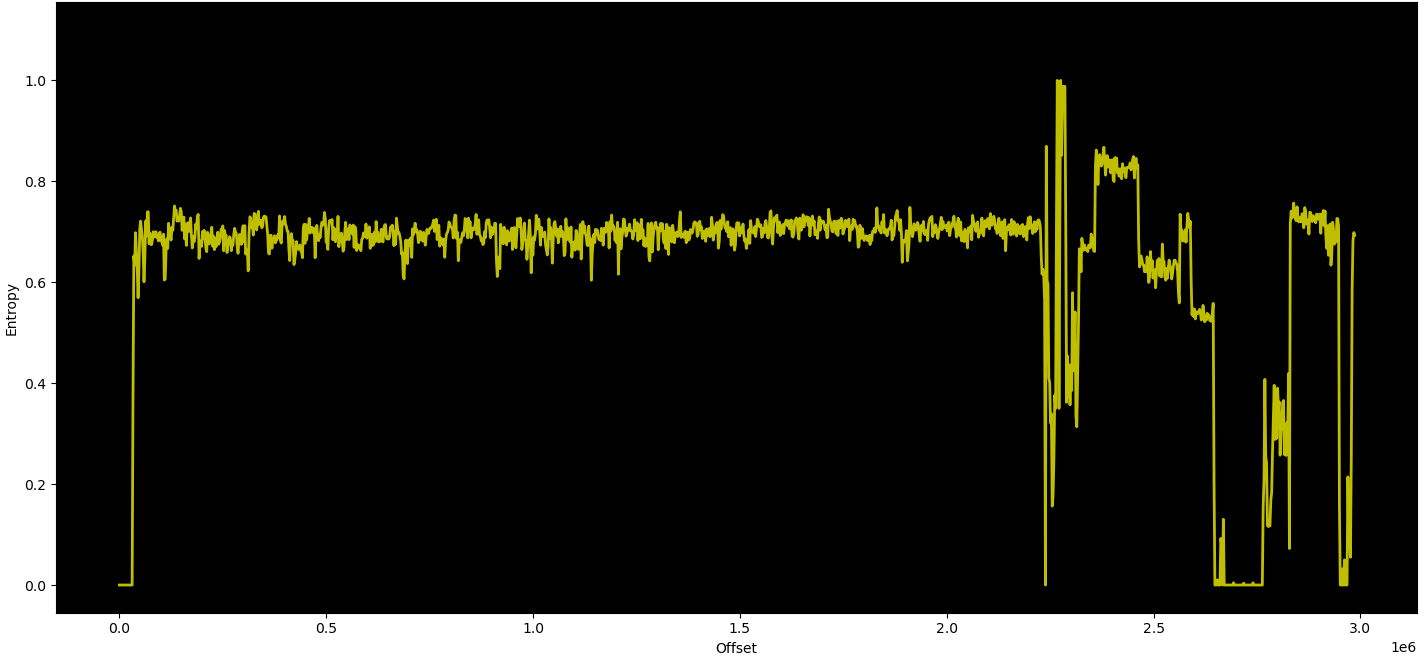
\includegraphics[scale=.35]{imagenes/entropia2.png}
     \label{fig:entropia2}
\end{figure}

\subsection{Exploring SquashFS: Hunting for Decryption Keys}

Within the file system (SquashFS), we identified a directory (/etc) containing seemingly interesting information. We focused on two files (\texttt{passwd.bak}, which we cracked using JohnTheRipper) and another file named \textbf{default\_config.xml}. Any configuration file can provide valuable insights into the system. When we try to view this XML file, we find:

\begin{minipage}{0.48\columnwidth}
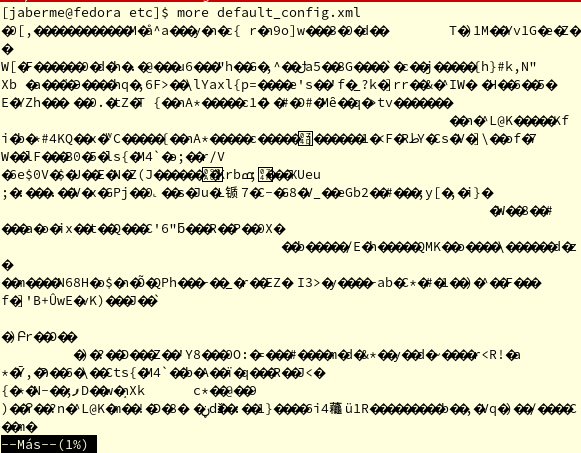
\includegraphics[scale=.3]{imagenes/defaultconfig.png}
\end{minipage}
\begin{minipage}{.5\columnwidth}
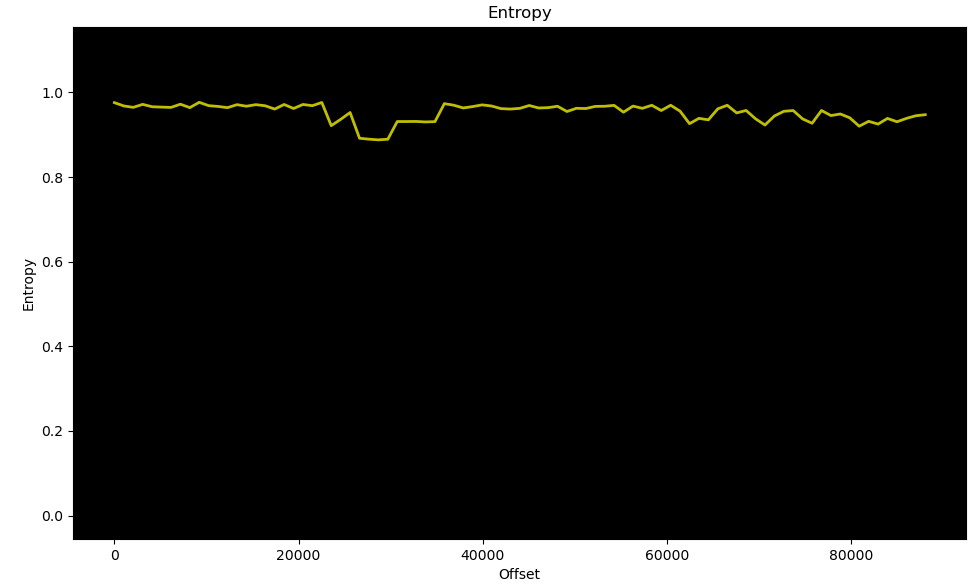
\includegraphics[scale=.25]{imagenes/entropy3.png}
\end{minipage}

If we explore /etc, we find a plethora of files to analyze, including binaries that seem related to the MT7628 SoC. However, our first target is \textbf{default\_config.xml}. When trying to open it (as shown in the figures above), we see that it is encrypted (unreadable characters) and has very high entropy (>0.7). If we’re interested in this file and cannot open it directly, the next step is to determine which programs in the operating system interact with this XML—because if we intercept them, we may be able to extract the key used to decrypt \textbf{default\_config.xml}.

\begin{verbatim}
grep -rnw ".." -e default_config.xml    
\end{verbatim}
\begin{itemize}
    \item \texttt{r}: recursive
    \item \texttt{n}: show line number
    \item \texttt{w}: search for whole word matches
\end{itemize}

The result points to just one reference, which is the library \textcolor{red}{\textbf{../lib/libcmm.so}}. Inside the router's file system, we locate this library that uses \texttt{default\_config.xml}. It is reasonable to assume that if this library accesses the file, then it must decrypt it at some point in order to process it.

\subsection{GHIDRA (https://ghidra-sre.org/)}

We will use Ghidra (see Figure~\ref{fig:Ghidra}) to perform reverse engineering on the \emph{shared object (.so)} file \textbf{\textcolor{red}{libcmm.so}}.

\begin{figure}[htpb]
     \caption{Ghidra}
     \centering
     
\includegraphics[scale=.35]{imagenes/Ghidra.png}
     \label{fig:Ghidra}
\end{figure}

The first step is to create a new project using the File → New Project menu. It must be configured as a \emph{non-shared project}. We then name it (e.g., \emph{AnalisisRouter}). We drag the library we want to analyze into the project (our .so shared object). The file \texttt{libcmm.so} is located inside the router's root file system, specifically in the /lib directory.

\begin{figure}[htpb]
     \caption{Ghidra: adding libcmm.so}
     \centering
     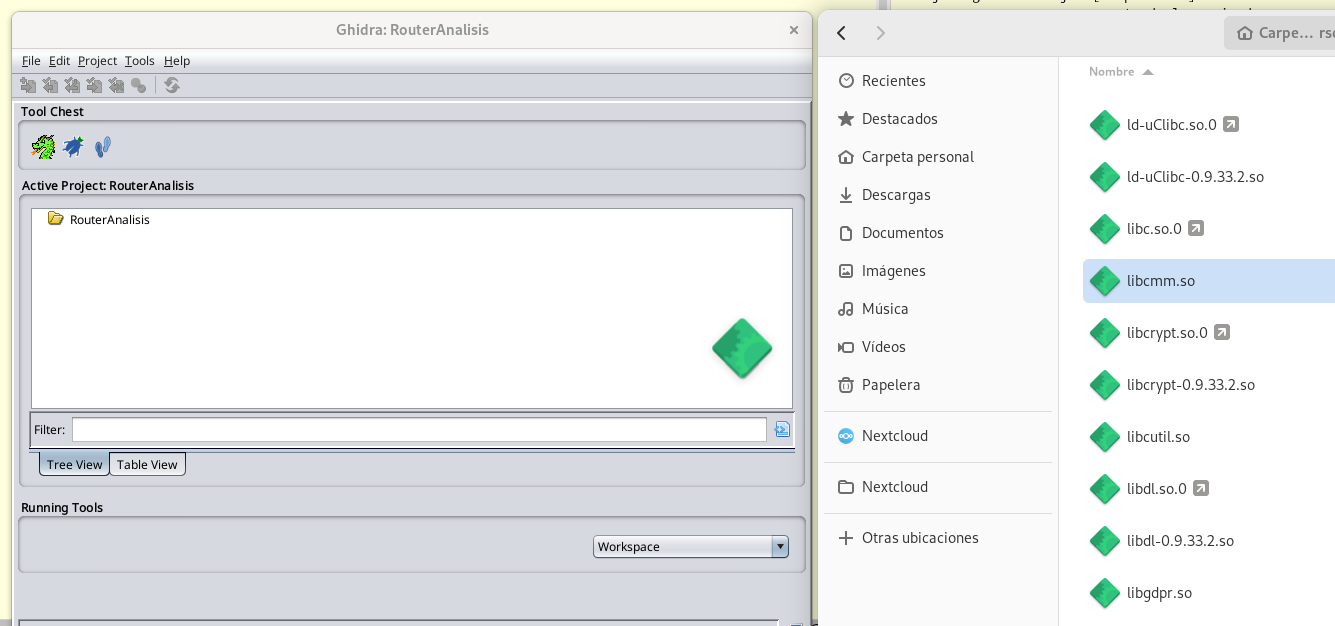
\includegraphics[scale=.35]{imagenes/RA.png}
     \label{fig:RA}
\end{figure}

During the import process, Ghidra recognizes the executable type automatically—we don't need to specify it manually, as shown in Figure~\ref{fig:RAfile}.

\begin{figure}[htpb]
     \caption{Ghidra: adding libcmm.so, format recognized.}
     \centering
     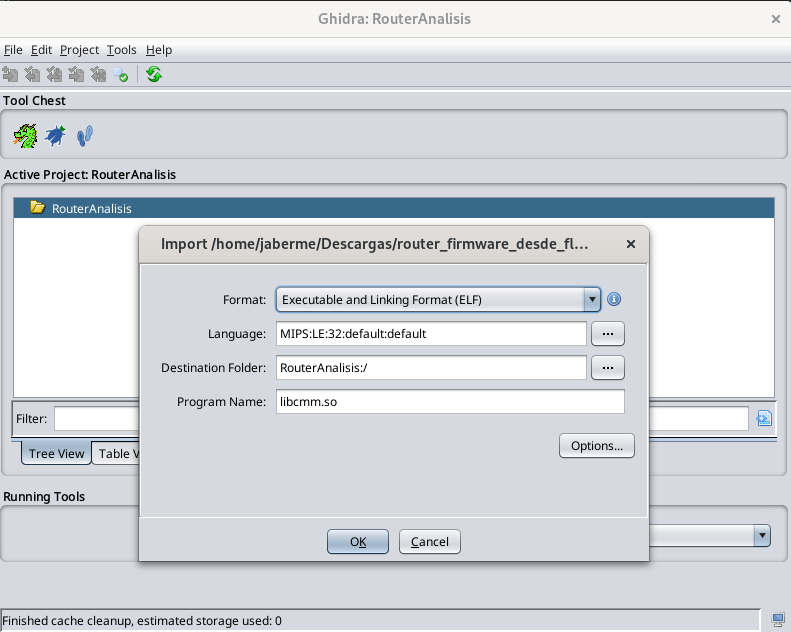
\includegraphics[scale=.5]{imagenes/RA_file.png}
     \label{fig:RAfile}
\end{figure}

The library is identified as a binary compiled for a 32-bit MIPS processor. Recall that the router's processor is a 32-bit MIPS operating at 500 MHz. Ghidra extracts detailed information, as shown in Figure~\ref{fig:RArquitectura}.

\begin{figure}[htpb]
     \caption{Ghidra: libcmm.so, MIPS 32-bit.}
     \centering
     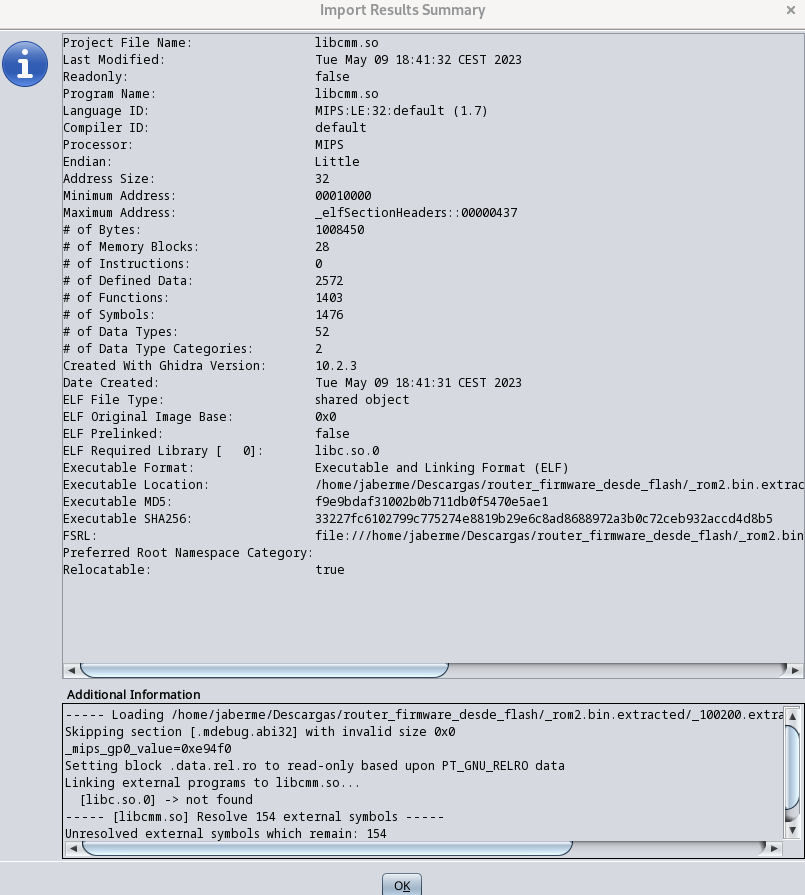
\includegraphics[scale=.5]{imagenes/RArquitecura.png}
     \label{fig:RArquitectura}
\end{figure}

Once the file is imported, we begin analysis by clicking on the dragon head icon (Figure~\ref{fig:RACabezaDragon}).

\begin{figure}[htpb]
     \caption{Ghidra: launching analysis with dragon icon.}
     \centering
     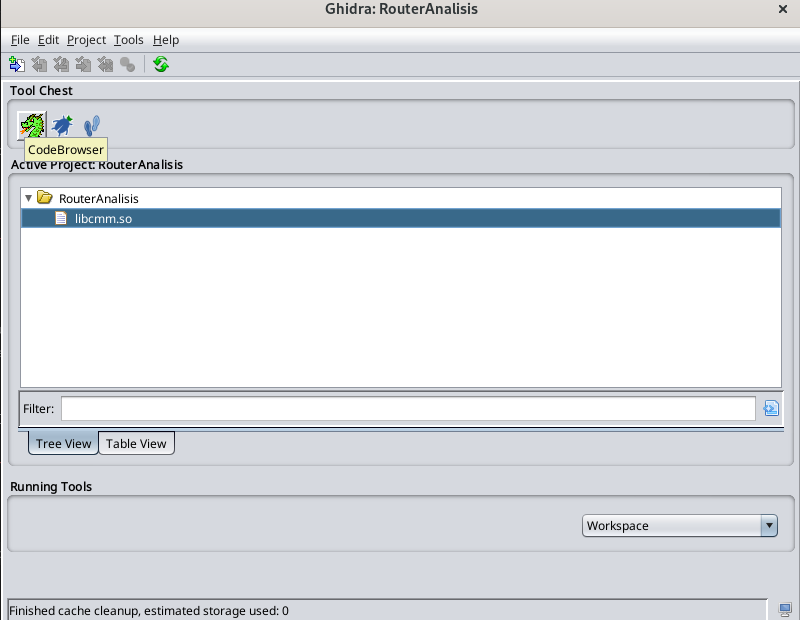
\includegraphics[scale=.5]{imagenes/RACabezaDragon.png}
     \label{fig:RACabezaDragon}
\end{figure}
To perform this analysis, the default options are sufficient. So we simply click \emph{Analyze} without changing any configuration (see Figure~\ref{fig:licmmAnalisis}).

\begin{figure}[htpb]
     \caption{Ghidra: libcmm.so, starting the analysis.}
     \centering
     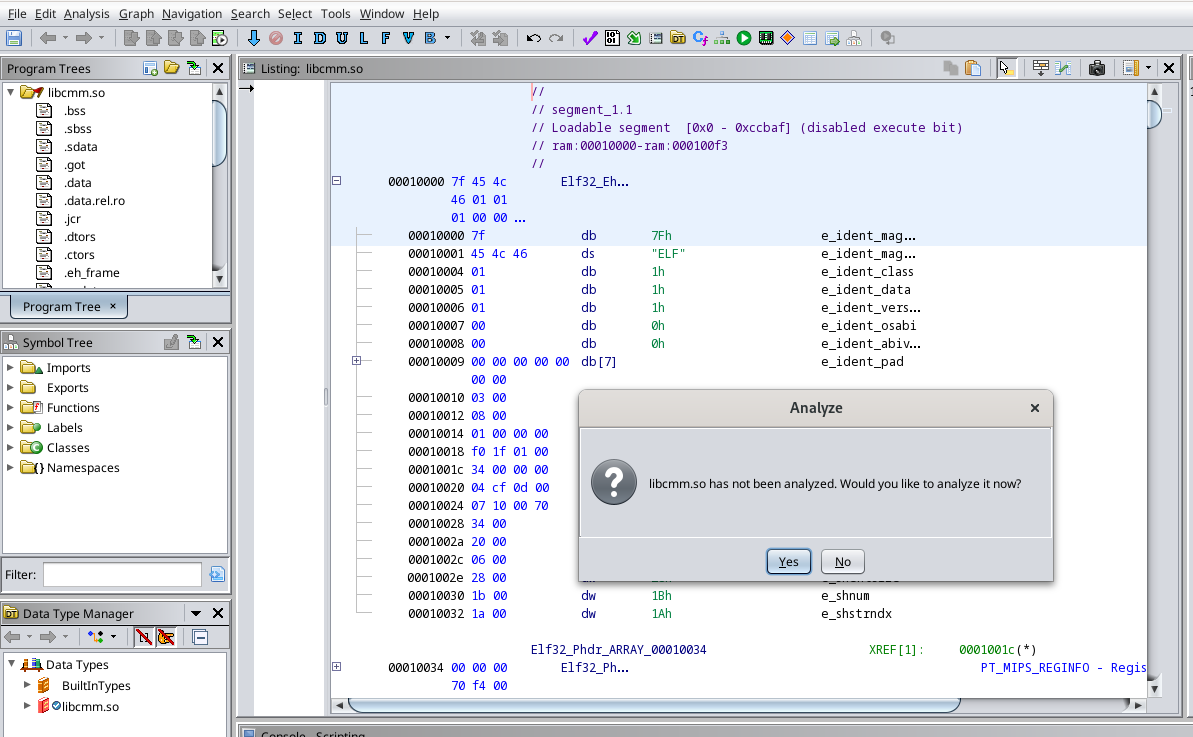
\includegraphics[scale=.35]{imagenes/licmmAnalisis.png}
     \label{fig:licmmAnalisis}
\end{figure}

In this first analysis, the default analyzers are useful. If needed, we could expand the range of analyzers, but for now, the built-in ones are enough. When the analysis starts, we must consider that it may take some time for Ghidra to display the \emph{disassembled} code of the library. Once it appears—and staying focused on our goal (we're looking for the relationship between this library and the encrypted file of interest, \emph{default\_config.xml})—our first move will be to search for this string inside the library’s code. That is, does \texttt{libcmm.so} explicitly reference \emph{default\_config.xml}? If so, and as we suspect, then the next question arises: if \texttt{libcmm.so} accesses \emph{default\_config.xml}, it must decrypt it first, right? And if so, it must contain the key to do so. That key is what we’re after, so we can read the contents of \emph{default\_config.xml}. Once the code has been analyzed, we search for the string via \textbf{Search → Program Text} (see Figure~\ref{fig:search}).

\begin{figure}[htpb]
     \caption{Ghidra: libcmm.so, searching for the string.}
     \centering
     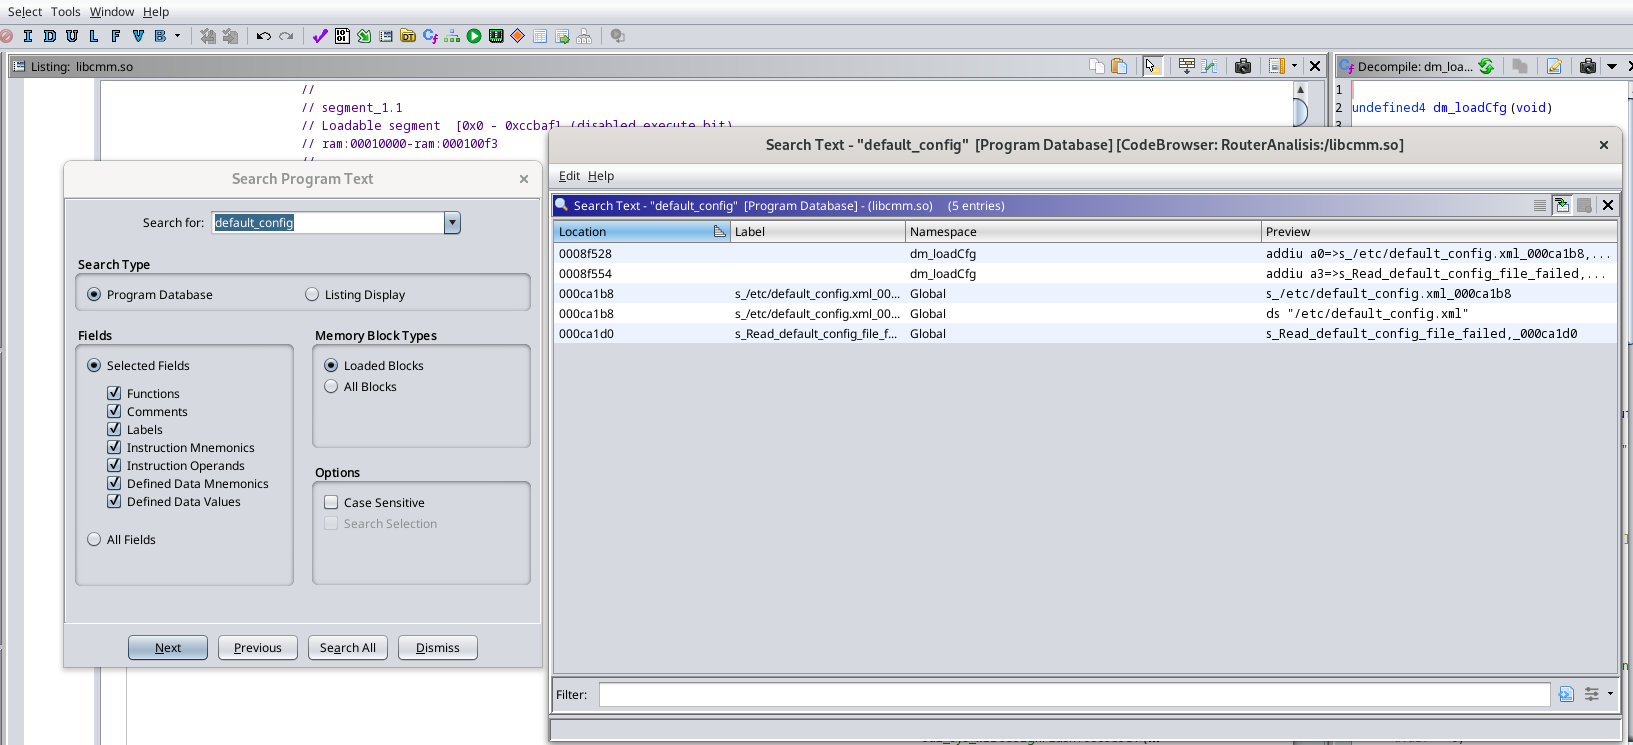
\includegraphics[scale=.25]{imagenes/search2.png}
     \label{fig:search}
\end{figure}

The first two results refer to code, so those are the first we’ll analyze. In these early lines of \emph{\textbf{dm\_loadCfg}}, we see the memory address where the code resides. Clicking on the first line takes us to that position (see Figure~\ref{fig:loadCfg}).

\begin{figure}[htpb]
     \caption{Ghidra: dm\_loadCfg}
     \centering
     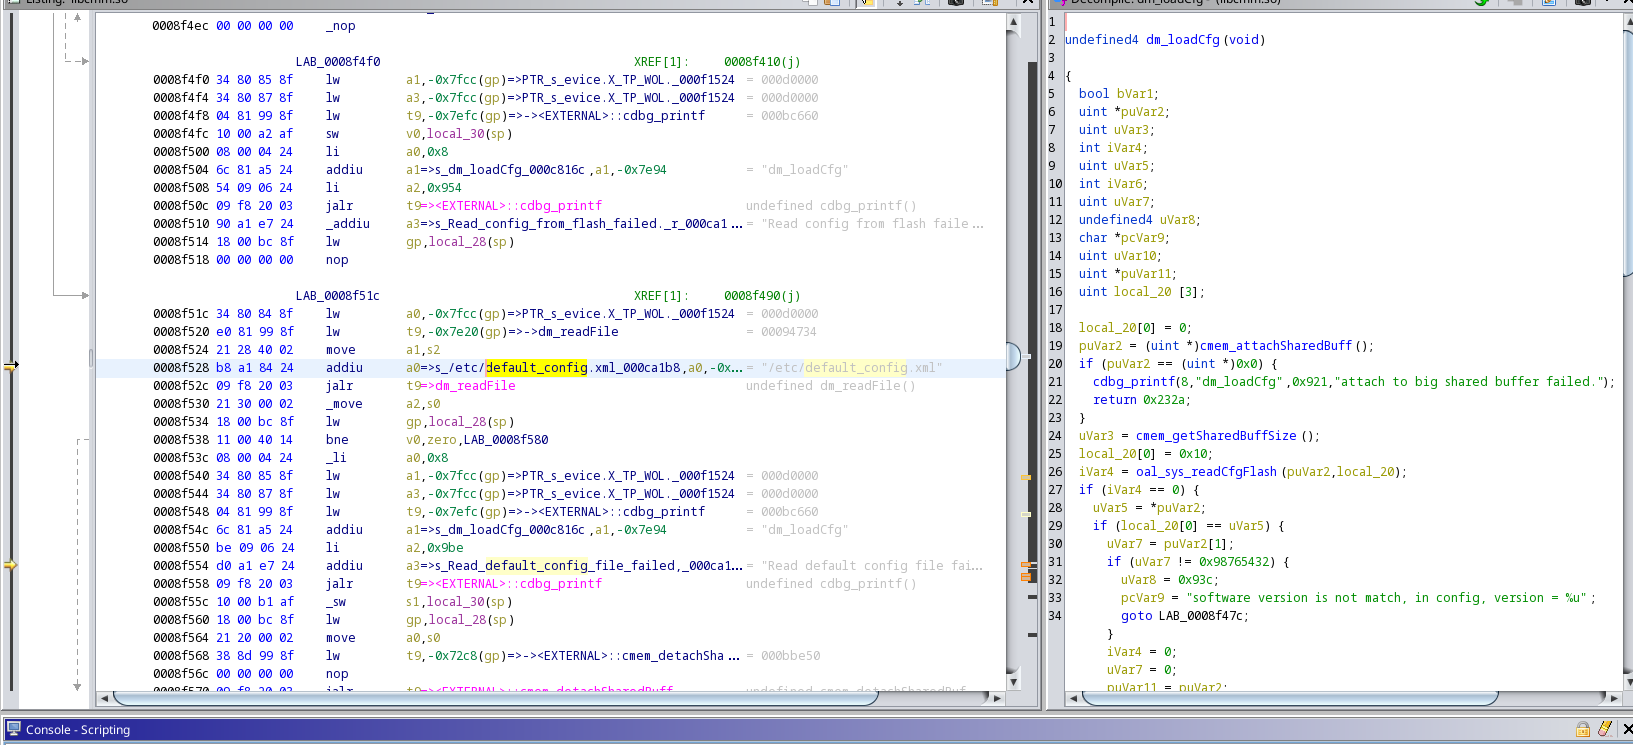
\includegraphics[scale=.25]{imagenes/loadCfg.png}
     \label{fig:loadCfg}
\end{figure}

As we navigate within the function \textbf{dm\_loadCfg} (shown in the panel on the right), we see a more readable pseudo-C representation of the function's logic. While analyzing it, we find it calls another function with a very telling name: \textbf{\emph{dm\_decryptFile}}. This function takes four parameters, but we don’t have much info on them yet. So, we click on the function name \textbf{\emph{dm\_decryptFile}} to try to understand how it performs decryption. In Figure~\ref{fig:dmDecryptFile}, at the beginning, we see 8 bytes copied from memory into a variable called \textbf{auStack28}. Then a function is called (\emph{cen\_desMinDo}—this is a \emph{wrapper}, meaning it mainly collects parameters and internally calls the decryption function, which resides in \texttt{libc.so}). It must be passed the key, and it looks like that key is stored in \texttt{auStack28}. The function has five parameters: the first four come from \texttt{dm\_decrypt}, and the final one is \textbf{auStack28}. So it seems very likely that this variable holds the decryption key.

\begin{figure}[htpb]
     \caption{Inside the function: dm\_loadCfg}
     \centering
     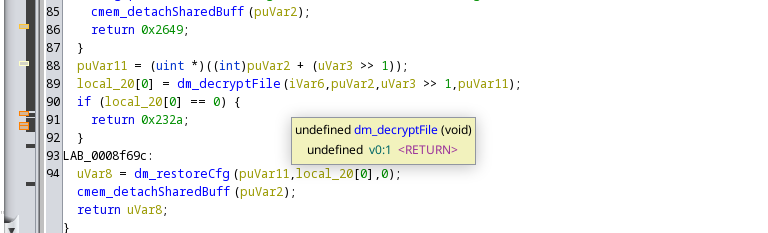
\includegraphics[scale=.25]{imagenes/dmDecrypt.png}
     \label{fig:dmdecrypt}
\end{figure}

\begin{figure}[htpb]
     \caption{Inside the function: dm\_decryptFile}
     \centering
     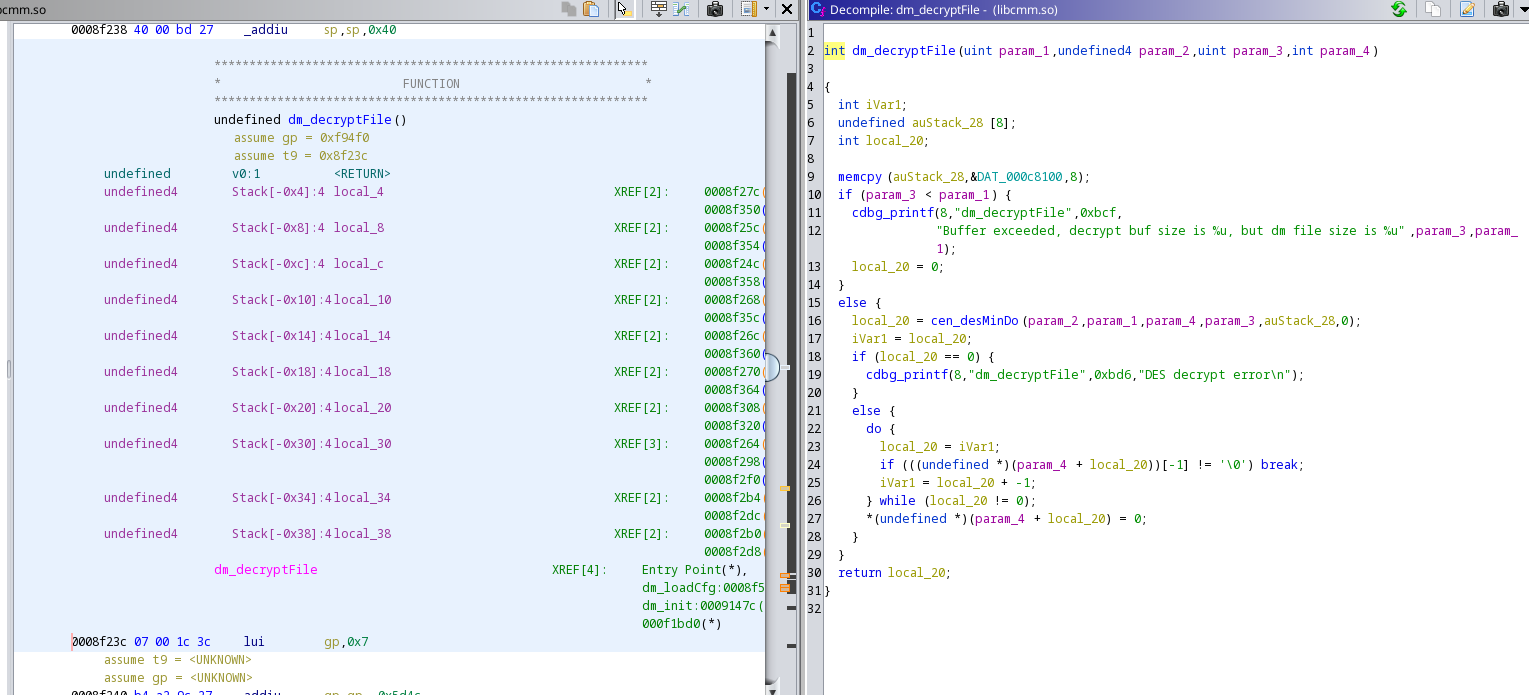
\includegraphics[scale=.25]{imagenes/decryptFile.png}
     \label{fig:dmDecryptFile}
\end{figure}

Logically, the next step is to check where \texttt{auStack28} gets its value (from which memory address). If we're right, that address should contain the decryption key. Figure~\ref{fig:memauStack28} shows how to access the memory area from which data is copied (via \texttt{memcpy}) into \texttt{auStack28}.

\begin{figure}[htpb]
     \caption{Accessing the memory area feeding auStack28}
     \centering
     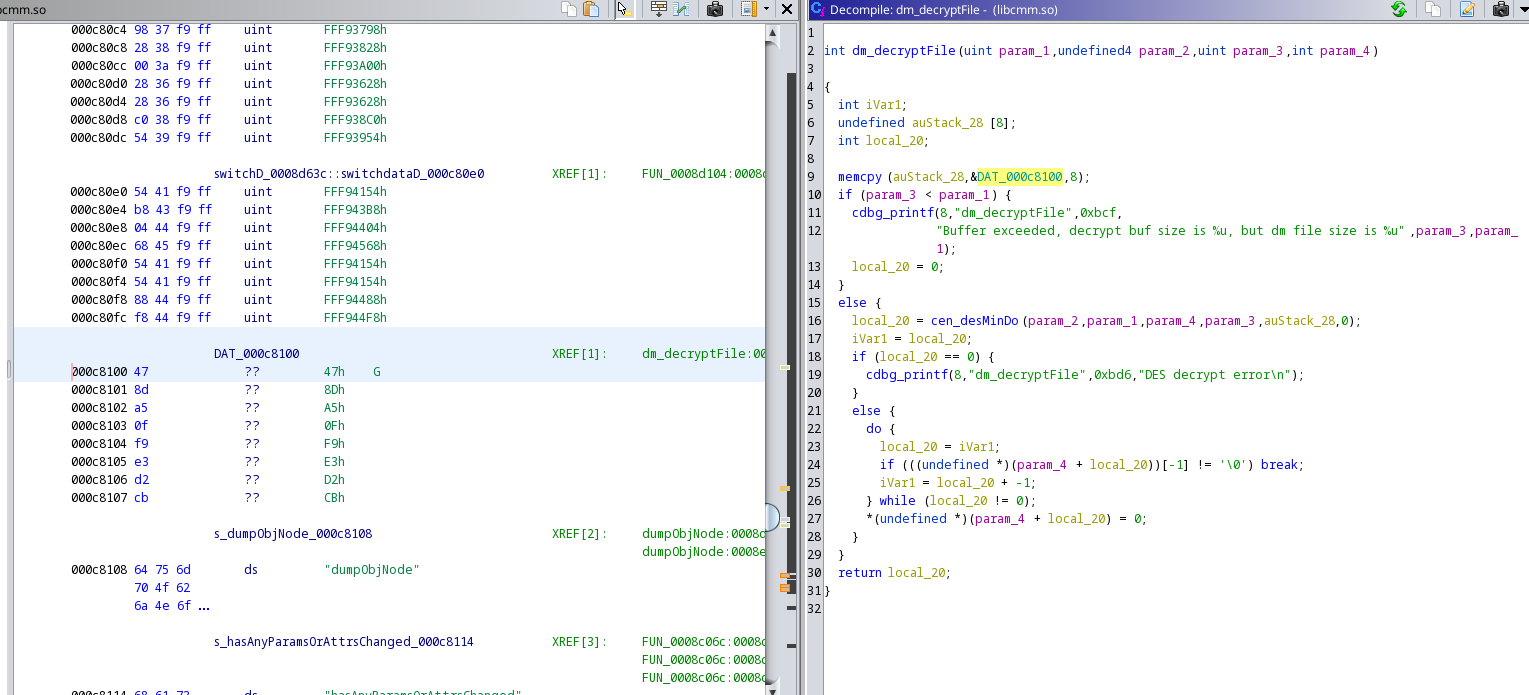
\includegraphics[scale=.35]{imagenes/memoria1.png}
     \label{fig:memauStack28}
\end{figure}

At that address in the program’s data area, we can see the 8 bytes copied into \texttt{auStack28}—\emph{\textbf{the decryption key}}. Thus, we’ve used reverse engineering techniques to uncover another backdoor and therefore a (\textcolor{red}{second vulnerability}).

\subsubsection{Decryption Key}

If we’re correct, we have found the key. To try decrypting \textbf{config\_default.xml}, we will use \textbf{openssl}.

\begin{tcolorbox}[colback=green!10]
    \textbf{openssl} is an open-source toolkit that provides a wide range of cryptographic utilities. It implements popular protocols and offers useful programming tools. It could be considered an essential toolkit, as it provides core algorithms for building secure cryptographic systems and SSL/TLS certificates.

    \textbf{The decryption key} we found is \textbf{\textcolor{red}{478DA50FF9E3D2CB}}. The \textbf{openssl} parameters we’ll use are:

    \begin{itemize}
        \item \textbf{-d} indicates decryption.
        \item \textbf{-des-ecb} specifies the DES algorithm in ECB mode (we saw this in function comments).
        \item \textbf{-K} specifies the key to use (\textbf{\textcolor{red}{478DA50FF9E3D2CB}}).
        \item \textbf{-in} indicates the file to decrypt.
        \item \textbf{-out} specifies the output file where the decrypted content will be written.
        \item \textbf{-provider} since DES-ECB is outdated and not included in modern \texttt{openssl enc} commands, we use this parameter to access the legacy provider.
    \end{itemize}
\end{tcolorbox}

The command we will use is:

\begin{tcolorbox}[colback=red!10]
openssl enc -d -des-ecb -in default\_config.xml -out decrypted.xml -K 478DA50FF9E3D2CB -provider legacy -provider default
\end{tcolorbox}

We get an error during decryption, but we can ignore it because the decrypted file still contains valid output (see Figure~\ref{fig:textoclaro}).

\begin{figure}[htpb]
     \caption{Decrypted file}
     \centering
     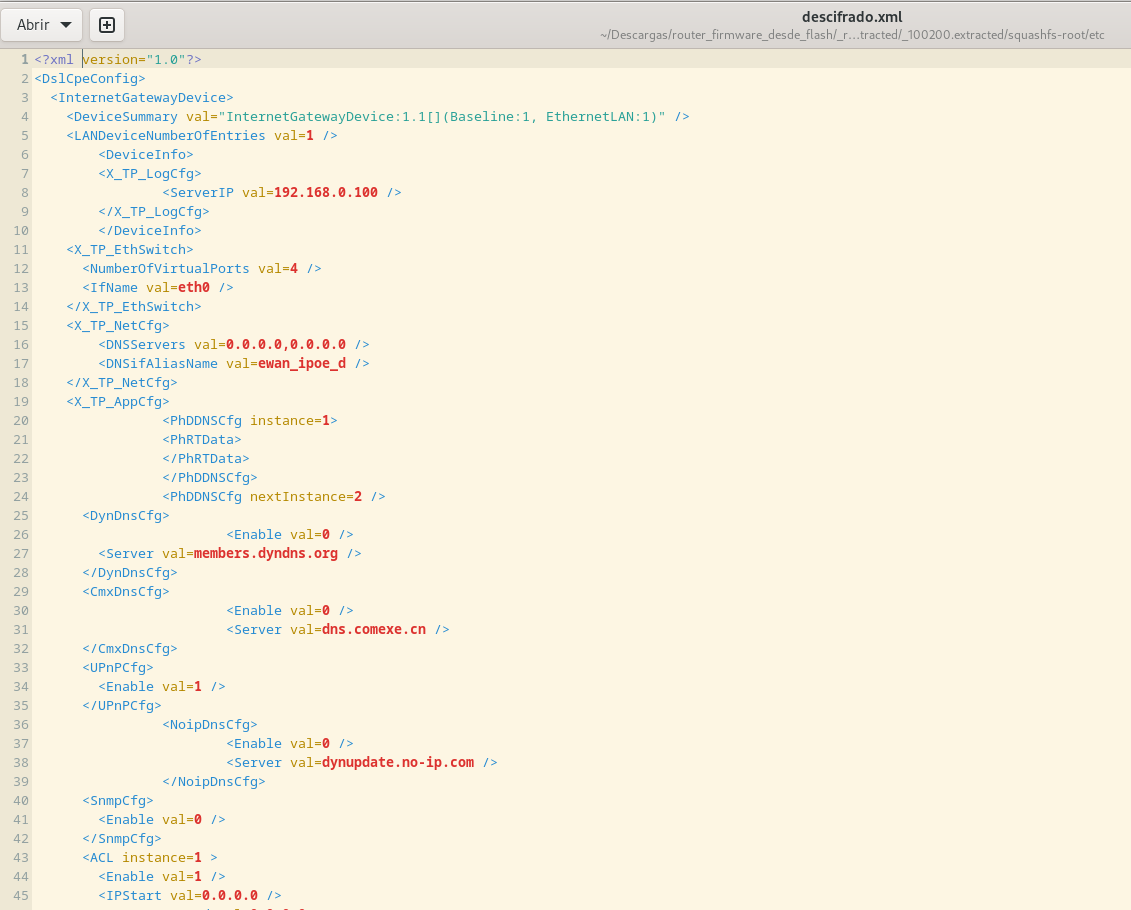
\includegraphics[scale=.45]{imagenes/textoclaro.png}
     \label{fig:textoclaro}
\end{figure}

The documentation includes the fully decrypted file to demonstrate that it contains sensitive information such as a voicemail PIN (123456) and a default cloud storage account (user: admin / password: admin) in the \texttt{<StorageService>} XML item.

By analyzing the decrypted file, we can uncover a significant amount of useful information.

\subsection{Vulnerabilities: System Calls}

At this point, several operations have been performed on the router:

\begin{itemize}
    \item The router’s firmware has been obtained through various methods.
    \item The Linux file system supporting the router has been extracted.
    \item A password hash was cracked using JohnTheRipper.
    \item Reverse engineering was performed on a shared library (\texttt{.so}) to extract the key used to encrypt a file containing sensitive information (default credentials, etc.).
\end{itemize}
In a more dedicated review with Ghidra, we identified a significant element affecting the router's security. In the left-hand panel of Ghidra, we find the \emph{Symbol Tree} window, which identifies modules, functions, classes—in short, everything used by \textbf{libcmm.so}. The \textbf{imports} folder lists functionality that resides outside \texttt{libcmm.so} (for example, that provided by the operating system). Which function should we focus on? There’s no fixed rule. However, in this case, what caught our attention is the appearance of \textbf{\textcolor{red}{system}} (see Figure~\ref{fig:system}). Using the \emph{execute} command, commands are launched from the router to the operating system (represented by the \texttt{system} function).

\begin{figure}[htpb]
     \caption{System}
     \centering
     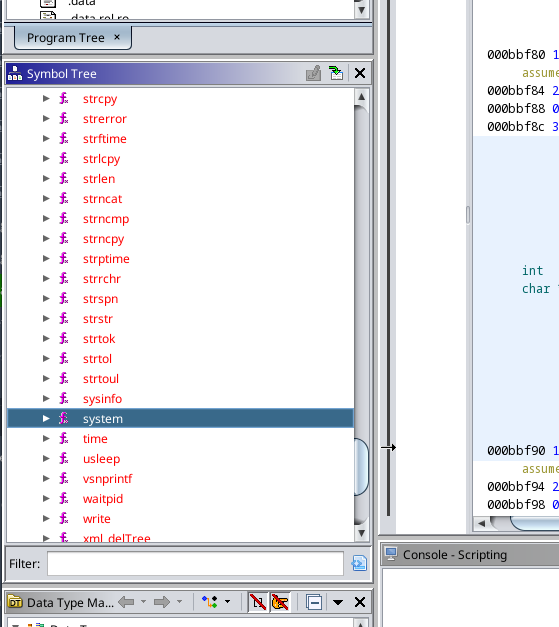
\includegraphics[scale=.45]{imagenes/system.png}
     \label{fig:system}
\end{figure}

In the next figure~\ref{fig:exec}, we can see in the \emph{Function Call Trees} window (which loads functions accessible from within \texttt{system}) two particularly interesting entries: the first is \textbf{updateFirmware}, used to update the router’s firmware, and the second is \textbf{util\_execSystem}, which allows access to the operating system that manages the router. Also, recall that any system call is executed as \textbf{root}; to verify this, just revisit the beginning of this document and check the output of the \texttt{whoami} command—it was \texttt{admin}. Executing system calls with this level of privilege is a security flaw and is therefore a (\textbf{\textcolor{red}{vulnerability}}).

\begin{figure}[htpb]
     \caption{System: execSystem function}
     \centering
     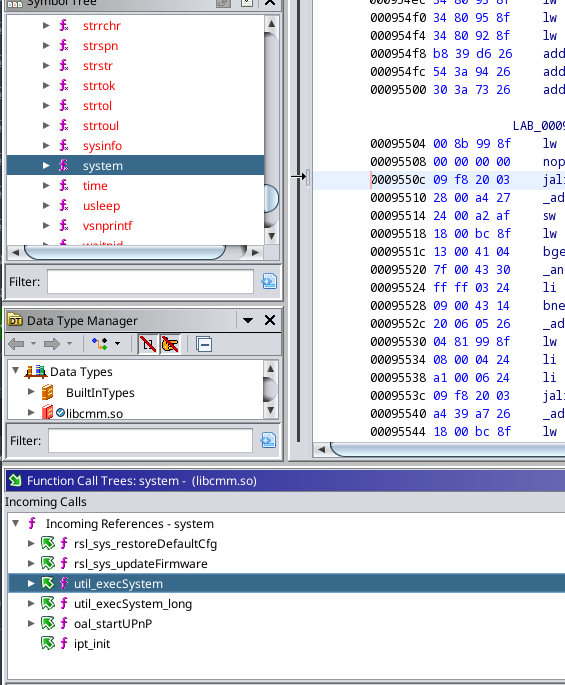
\includegraphics[scale=.4]{imagenes/exec.png}
     \label{fig:exec}
\end{figure}

If we navigate the function call tree, we will see dozens and dozens of system calls through \texttt{util\_execSystem}. Selecting one such function, for example, \textbf{\textcolor{red}{oal\_ipt\_addBridgeIsolationRules}}, we can view its decompiled code and observe how it makes system calls. The function receives parameters and issues a system command—specifically \texttt{iptables}—see Figure~\ref{fig:bridge}. This command is configured to receive the IP address through those parameters. It is very likely that this function is invoked from the router’s web interface, where the user inputs the IP address through the admin panel.

\begin{figure}[htpb]
     \caption{Function oal\_ipt\_addBridgeIsolationRules}
     \centering
     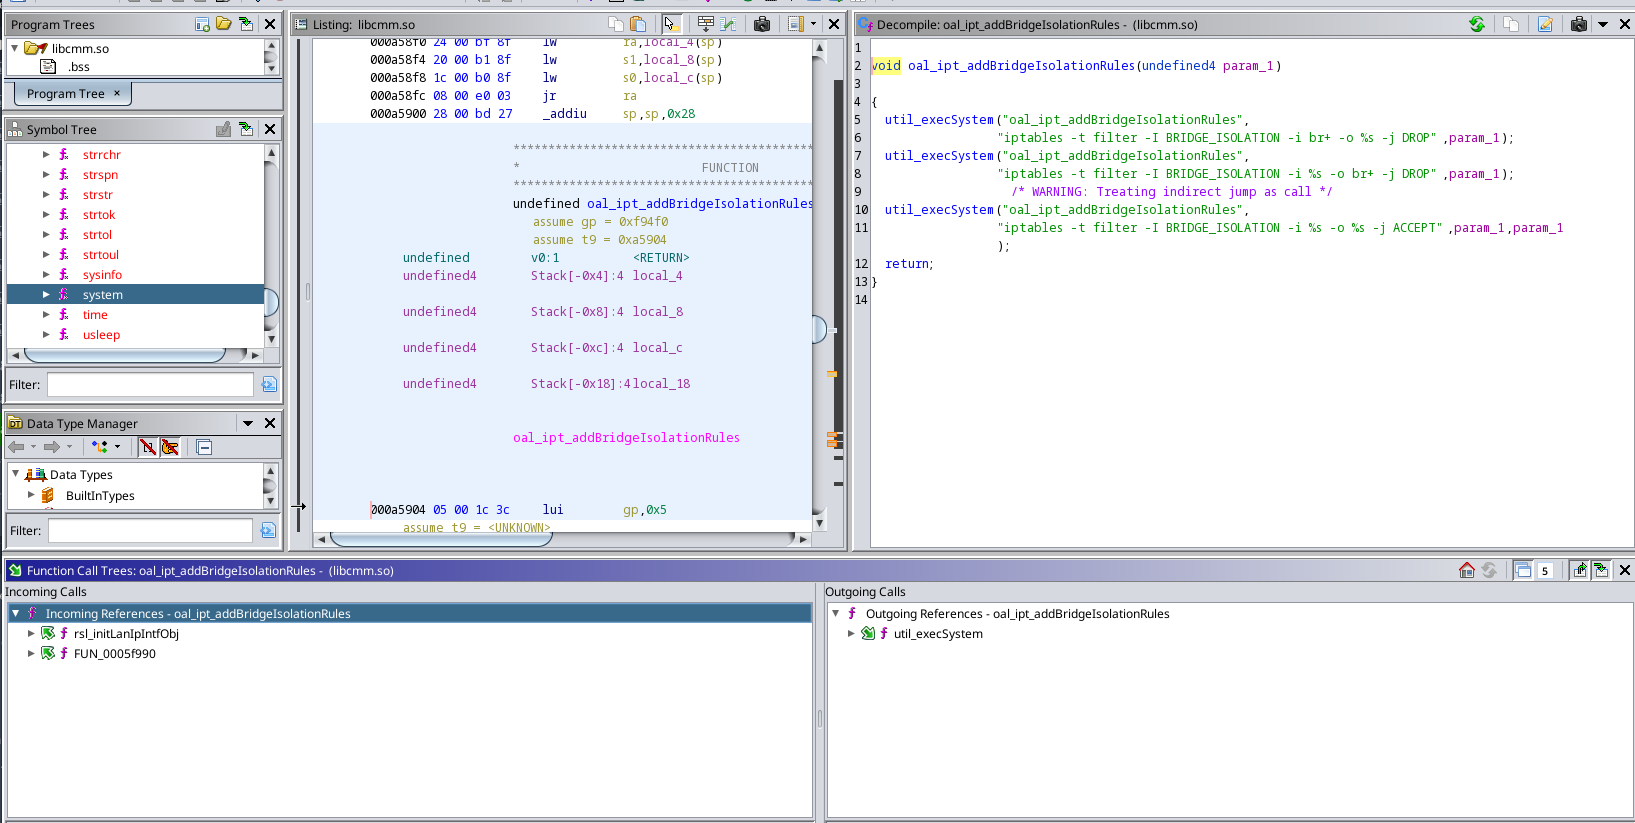
\includegraphics[scale=.30]{imagenes/bridge.png}
     \label{fig:bridge}
\end{figure}

The user, from the router’s admin page, specifies the IP address, and this web interface sends the IP (\textbf{\textcolor{red}{WITHOUT CHECKING (without sanitizing) whether it is actually a valid IP address}}). This IP address is embedded in an \texttt{iptables} command and sent to the router’s operating system (as user \texttt{admin}, let’s not forget).

\subsubsection{Command Injection}

What would happen if, instead of a valid IP address, a specific command were sent to the router? But of course, how can we \emph{inject} data through the web interface if it doesn't allow free-form input? The answer is simple: we need to intercept what the browser sends to the router:

\begin{itemize}
    \item Connect your computer to the same network as the router.
    \item Access its IP through a browser.
    \item You receive the configuration page.
    \item Install a tool such as \textbf{Burp Suite} on your computer.
    \item All data from the web to the router passes through this \emph{proxy}.
    \item That data is captured by \textbf{BurpSuite}; we then modify the parameter sent from the web form to the router (since we’ve paused it in our proxy) and send it manually.
    \item The router executes our command instead of the one it was programmed to execute.
    \item Web-based system access has been achieved.
\end{itemize}

\begin{figure}[htpb]
     \caption{Command injection}
     \centering
     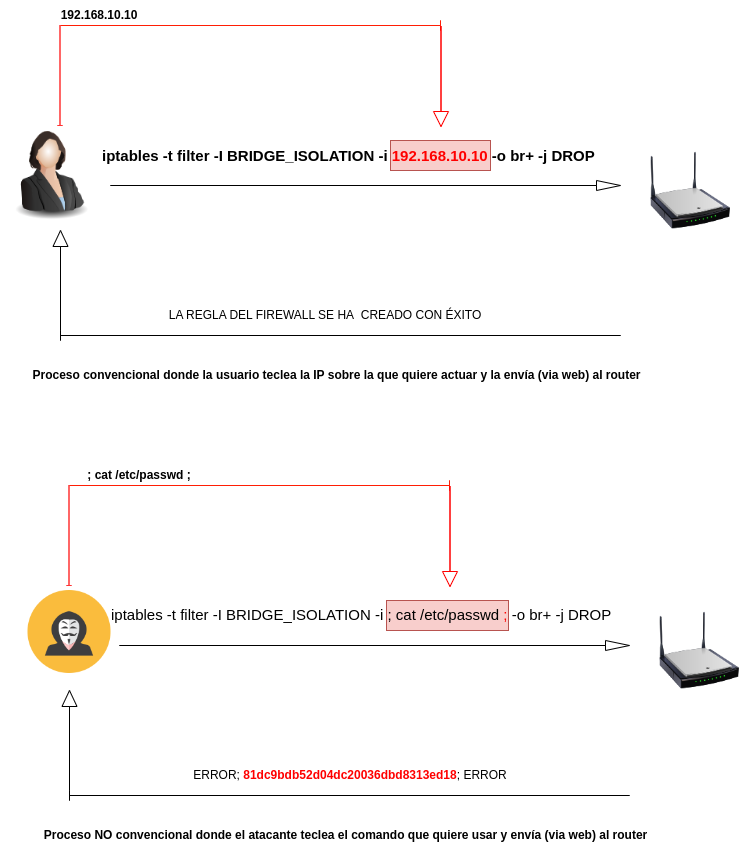
\includegraphics[scale=.65]{imagenes/tfg.png}
     \label{fig:tfg}
\end{figure}

The way to do what is illustrated in Figure~\ref{fig:tfg} is by intercepting communications between the browser and the router’s web server using \textbf{BurpSuite} or similar tools. Figure~\ref{fig:burp} shows BurpSuite acting as a proxy. It intercepts communications and allows you to modify parameters. When we submit an IP address in a web form to the router, instead of letting it go directly, we route it through \textbf{BurpSuite}, where we replace the IP with a command, putting us in a position to take full control of the router.

\begin{figure}[htpb]
     \caption{BurpSuite}
     \centering
     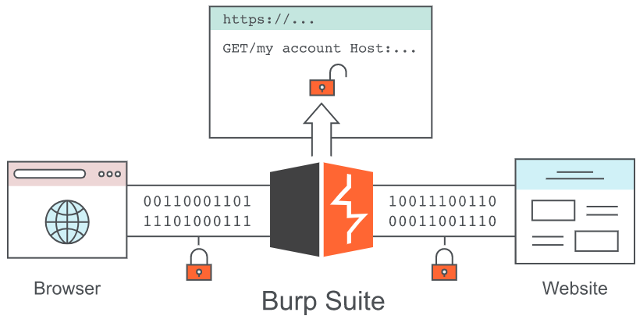
\includegraphics[scale=1]{imagenes/burp_suite.png}
     \label{fig:burp}
\end{figure}

\section{More Resources}

\begin{tcolorbox}[enhanced, dropshadow, title=Full-on Reversing, colback=blue!10]
    \begin{itemize}
        \item \href{https://voidstarsec.com/blog/intro-to-embedded-part-1}{Introduction to Reverse Engineering in Embedded Devices}
    \end{itemize}
\end{tcolorbox}

\printbibliography

\end{document}
